\documentclass[12pt]{article}
\usepackage[utf8]{inputenc}
\usepackage[vietnamese]{babel}
\usepackage[T5]{fontenc}
\usepackage{amsmath}
\usepackage{amsfonts}
\usepackage{float}
\usepackage{indentfirst}
\usepackage{fancyhdr}
\usepackage{titlesec}
\usepackage{makeidx}
\usepackage{graphicx}
\usepackage{setspace}
\usepackage{xurl}
\usepackage[colorlinks=true,linkcolor=blue,citecolor=red,urlcolor=blue]{hyperref}
\usepackage[top=.75in, left=.75in, right=.75in, bottom=1in]{geometry}
\usepackage{listings}
\usepackage{xcolor}
\usepackage{tabularx}
\usepackage{booktabs}
\usepackage{caption}
\usepackage{microtype}

\makeindex

% Paragraph Spacing, Indentation, and Overflow Protection
\setlength{\parskip}{5pt}
\setlength{\parindent}{0.6cm}
\emergencystretch 3em
\hfuzz=1pt
\vfuzz=1pt

% Line spacing 1.2
\renewcommand{\baselinestretch}{1.2}

% Code Listing Styling
\definecolor{codegreen}{rgb}{0,0.6,0}
\definecolor{codegray}{rgb}{0.5,0.5,0.5}
\definecolor{codepurple}{rgb}{0.58,0,0.82}
\definecolor{backcolour}{rgb}{0.97,0.97,0.97}

\lstdefinestyle{mystyle}{
    backgroundcolor=\color{backcolour},   
    commentstyle=\color{codegreen},
    keywordstyle=\color{blue}\bfseries,
    numberstyle=\tiny\color{codegray},
    stringstyle=\color{codepurple},
    basicstyle=\ttfamily\footnotesize,
    breakatwhitespace=false,         
    breaklines=true,                 
    captionpos=b,                    
    keepspaces=true,                 
    numbers=none,                    
    numbersep=5pt,                  
    showspaces=false,                
    showstringspaces=false,
    showtabs=false,                  
    tabsize=2,
    frame=single,
    rulecolor=\color{black!20}
}
\lstset{style=mystyle}

% YAML language support for listings
\lstdefinelanguage{yaml}{
  keywords={true,false,null,y,n},
  keywordstyle=\color{blue}\bfseries,
  basicstyle=\ttfamily\footnotesize,
  sensitive=false,
  comment=[l]{\#},
  morecomment=[s]{/*}{*/},
  commentstyle=\color{codegreen}\ttfamily,
  stringstyle=\color{codepurple}\ttfamily,
  moredelim=[l][\color{blue}]{\&},
  moredelim=[l][\color{blue}]{*},
  moredelim=**[il][\color{red}\bfseries{:}\ ]{: \ },
  morestring=[b]',
  morestring=[b]"
}

% Rename bibliography title to "Tài liệu tham khảo"
\addto\captionsvietnamese{
  \renewcommand{\refname}{Tài liệu tham khảo}
  \renewcommand{\bibname}{Tài liệu tham khảo}
}

% Course and Report Metadata
\newcommand{\reportname}{Triển khai và Vận hành Hạ tầng Điện toán Đám mây}
\newcommand{\reporttitle}{Đồ án 2: Xây dựng Đám mây Riêng trên nền tảng OpenStack}

\newcommand{\studentname}{
    \textbf{Ngô Tấn Tài} -- \texttt{23127470} \\
    \textbf{Nguyễn Tấn Lộc} -- \texttt{23127406} \\
    \textbf{Hồ Minh Dũng} -- \texttt{23127174} \\
}

\newcommand{\teachername}{
    Cô Chung Thùy Linh\\
    Thầy Lê Ngọc Sơn\\
}

% Header and Footer
\setlength{\headheight}{29.5pt}
\pagestyle{fancy}
\fancyhead{}
\lhead{\small \textbf{CSC11006} --- \reporttitle}
\rhead{\small \thepage}
\fancyfoot{}

% Document Body
\begin{document}

\pagenumbering{alph}
\begin{titlepage}
\begin{center}

\textbf{\large ĐẠI HỌC QUỐC GIA THÀNH PHỐ HỒ CHÍ MINH}\\[0.15cm]
\textbf{\large TRƯỜNG ĐẠI HỌC KHOA HỌC TỰ NHIÊN}\\[0.15cm]
\textbf{\large KHOA CÔNG NGHỆ THÔNG TIN}\\[0.3cm]

\vspace{0.1cm}

\includegraphics[width=5.6cm]{img/hcmus-logo.png}
\vspace{0.2cm}

\rule{\textwidth}{1.2pt} \\[0.3cm]
{\huge \textbf{\reporttitle}} \\[0.25cm]
{\large \textbf{Môn học: \reportname}} \\[0.15cm]
\rule{\textwidth}{1.2pt} \\[0.6cm]

\begin{minipage}[t]{0.50\textwidth}
\begin{flushleft} \large
\emph{Sinh viên thực hiện:}\\
\studentname
\end{flushleft}
\end{minipage}
~
\begin{minipage}[t]{0.45\textwidth}
\begin{flushleft} \large
\emph{Giảng viên hướng dẫn:}\\
\teachername
\end{flushleft}
\end{minipage}

\vfill
{\large \textbf{Thành phố Hồ Chí Minh, Tháng 8/2026}}

\end{center}
\end{titlepage}


\newpage
\pagenumbering{roman}
\tableofcontents
\newpage
\pagenumbering{arabic}

\section{Tổng quan \& Thông số Môi trường Thực nghiệm}

\subsection{Mục tiêu \& Phạm vi Đồ án}
Trong khuôn khổ đồ án môn học, nhóm chúng em tập trung triển khai và vận hành một hệ thống hạ tầng đám mây riêng (Private Cloud) hoàn chỉnh dựa trên nền tảng mã nguồn mở OpenStack thông qua công cụ tự động hóa DevStack. Mục tiêu cốt lõi của nhóm là trực tiếp khảo sát, thực hành và làm chủ các nguyên lý kỹ thuật hạ tầng đám mây (Cloud Engineering), bao gồm mô hình Hạ tầng dưới dạng Dịch vụ (IaaS), công nghệ mạng ảo hóa điều khiển bằng phần mềm (SDN), quản lý vòng đời lưu trữ khối/đối tượng và tự động hóa điều phối hạ tầng dưới dạng mã (IaC).

Quá trình thực nghiệm của nhóm được chia thành 5 phân hệ kỹ thuật (Module) cụ thể:
\begin{itemize}
    \item \textbf{Dịch vụ cốt lõi \& Quản lý vòng đời (Module 1):} Khảo sát, kiểm thử và vận hành các dịch vụ OpenStack thông qua giao diện Web Horizon và công cụ dòng lệnh OpenStack CLI.
    \item \textbf{Phân đoạn \& Cô lập mạng Tenant (Module 2):} Xây dựng cấu trúc mạng đa tầng phân lập gồm mạng ngoại vi (Provider Network), vùng mạng DMZ, mạng nội bộ Private và bộ định tuyến ảo L3 Router.
    \item \textbf{Máy ảo đa Card mạng \& Cung cấp dịch vụ (Module 3):} Khởi tạo máy ảo gắn đồng thời 2 card mạng (Dual-NIC), xử lý triệt để bài toán định tuyến bất đối xứng (Asymmetric Routing) trong nhân Linux, gán Floating IP và triển khai dịch vụ web công khai.
    \item \textbf{Lưu trữ Bền vững \& Phục hồi sau thảm họa (Module 4):} Quản trị tài nguyên tĩnh phi cấu trúc bằng Swift Object Storage và ổ đĩa khối bền vững với Cinder Block Storage; thực hiện quy trình tạo Snapshot và khôi phục dữ liệu nguyên vẹn trên máy ảo độc lập.
    \item \textbf{Tự động hóa Khai báo Hạ tầng với Heat (Module 5):} Soạn thảo mẫu điều phối Heat Orchestration Template (HOT) kết hợp kịch bản Cloud-Init để tự động hóa toàn bộ vòng đời từ cấp phát hạ tầng đến khởi chạy ứng dụng web.
\end{itemize}

\subsection{Môi trường Thực nghiệm Lab}
Để phục vụ quá trình thực nghiệm, nhóm chúng em triển khai hệ thống OpenStack theo mô hình All-in-One trên một máy ảo chạy trong môi trường ảo hóa lồng nhau (Nested KVM) thuộc máy chủ Proxmox VE. Thông số cấu hình chi tiết được tổng hợp tại Bảng~\ref{tab:env_specs}.

\begin{table}[H]
\centering
\small
\begin{tabular}{|l|p{9.2cm}|}
\hline
\textbf{Thông số} & \textbf{Cấu hình / Giá trị thực tế} \\ \hline
Nền tảng ảo hóa & Proxmox VE (Nested Hardware Virtualization KVM)~\cite{kvm_paper} \\ \hline
Hệ điều hành Host & Ubuntu Server 24.04.4 LTS (\texttt{noble}), Linux Kernel 6.8 \\ \hline
Tài nguyên phần cứng & 4 vCPUs, 22 GiB RAM, 73 GiB NVMe Root Disk, 8 GiB Swap \\ \hline
Nhánh DevStack & \nolinkurl{stable/2026.1} (Commit: \nolinkurl{da2f4d73f5ad74fc8ecfbe15bd7e20f6b0982dbb}) \\ \hline
Kiểu ảo hóa Hypervisor & \texttt{LIBVIRT\_TYPE=kvm} (Tăng tốc phần cứng QEMU/KVM) \\ \hline
Dịch vụ mở rộng kích hoạt & Heat Orchestration, Heat Dashboard, Swift Object Storage \\ \hline
IP Host / Cổng kết nối & \texttt{192.168.2.10} / NetBird Overlay Mesh VPN Gateway \\ \hline
Giao diện quản trị Web & \url{https://openstack.net.selfhost.io.vn/dashboard} \\ \hline
\end{tabular}
\caption{Thông số môi trường máy chủ và cấu hình triển khai DevStack.}
\label{tab:env_specs}
\end{table}

\noindent \textbf{Giải trình kỹ thuật về phiên bản Hệ điều hành:} Mặc dù tài liệu đề bài ban đầu gợi ý Ubuntu 22.04 LTS, nhóm chúng em quyết định lựa chọn nền tảng Ubuntu 24.04.4 LTS (\texttt{noble}). Quyết định này bắt nguồn từ yêu cầu kỹ thuật thực tế của nhánh DevStack chính thức mới nhất (\nolinkurl{stable/2026.1}), vốn đòi hỏi môi trường Python 3.12 và các gói thư viện OpenStack phụ thuộc chỉ được hỗ trợ toàn diện trên phiên bản Ubuntu 24.04.

\subsection{Phân công Trách nhiệm \& Quy tắc Cô lập Tài nguyên}
Để đảm bảo quá trình thực hành nhóm diễn ra nhịp nhàng, tránh xung đột tài nguyên trên máy chủ DevStack All-in-One dùng chung, nhóm chúng em đã thống nhất bảng phân công nhiệm vụ cụ thể (Bảng~\ref{tab:team_assignment}) cùng các quy tắc vận hành chặt chẽ.

\begin{table}[H]
\centering
\small
\begin{tabularx}{\linewidth}{|l|l|>{\raggedright\arraybackslash}X|c|}
\hline
\textbf{Thành viên} & \textbf{Vai trò} & \textbf{Nhiệm vụ Phụ trách} & \textbf{Đóng góp} \\ \hline
Ngô Tấn Tài (23127470) & Trưởng nhóm & & 100\% \\ \hline
Nguyễn Tấn Lộc (23127406) & Thành viên & & 100\% \\ \hline
Hồ Minh Dũng (23127174) & Thành viên & & 100\% \\ \hline
\end{tabularx}
\caption{Bảng phân công trách nhiệm và tỷ lệ đóng góp của các thành viên trong nhóm.}
\label{tab:team_assignment}
\end{table}

\noindent \textbf{Quy tắc đặt tên tài nguyên (Naming Conventions):} Các thành viên trong nhóm thống nhất bắt buộc sử dụng tiền tố theo từng module (ví dụ: \texttt{m2-dmz-net}, \texttt{m3-web-server}, \texttt{m4-data-volume}, \texttt{m5-server}). Quy tắc này giúp ngăn ngừa triệt để việc ghi đè cấu hình và giúp quá trình nghiệm thu, dọn dẹp tài nguyên diễn ra độc lập mà không ảnh hưởng đến phần việc của nhau.


\newpage

\section{Kiến trúc Hệ thống \& Cấu trúc Tô-pô Mạng}

\subsection{Phân tầng Kiến trúc OpenStack}
Hệ thống OpenStack vận hành theo mô hình kiến trúc phân tán dạng hướng dịch vụ (Microservices), trong đó các dịch vụ độc lập giao tiếp với nhau thông qua giao diện lập trình ứng dụng RESTful HTTP APIs và hàng đợi thông điệp RabbitMQ, dưới sự chứng thực tập trung của dịch vụ định danh Keystone~\cite{openstack_arch, devstack_docs} (Hình~\ref{fig:sys_architecture}).

\begin{figure}[H]
\centering
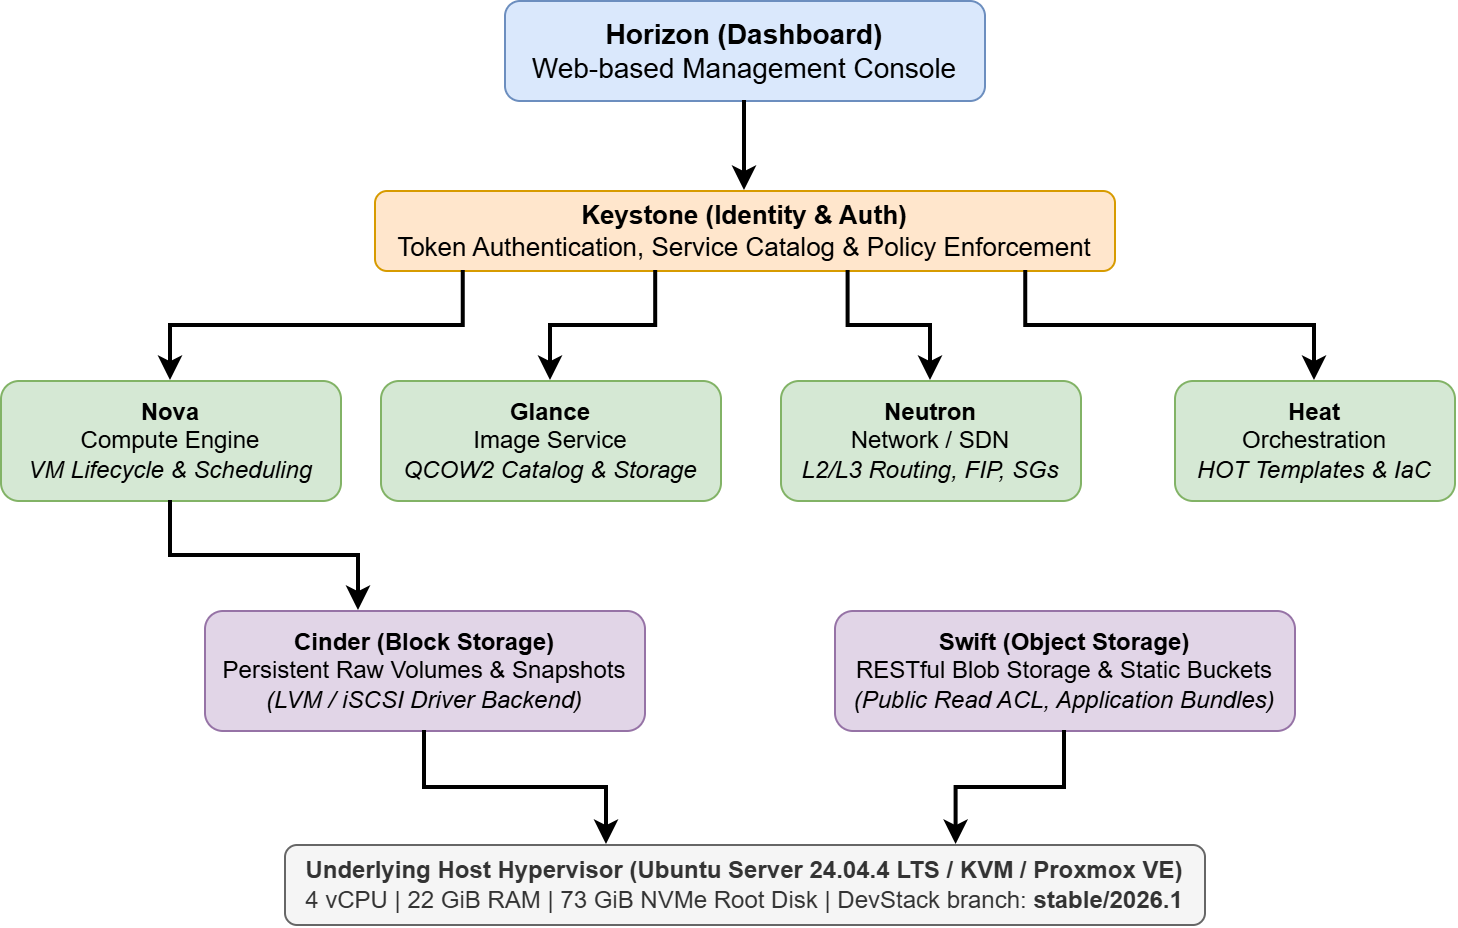
\includegraphics[width=0.92\linewidth]{img/openstack_architecture.png}
\caption{Kiến trúc phân tầng và luồng tương tác giữa các vi dịch vụ trong hệ thống OpenStack.}
\label{fig:sys_architecture}
\end{figure}

Trong phạm vi triển khai của đồ án, các khối dịch vụ cốt lõi đảm nhận các vai trò kỹ thuật cụ thể như sau:
\begin{enumerate}
    \item \textbf{Xác thực \& Định danh (Keystone):} Xác thực các yêu cầu API, phát hành mã token có phạm vi truy cập (Scoped Token) và phân giải URL endpoint của các dịch vụ trong mạng nội bộ cũng như mạng quản trị.
    \item \textbf{Quản lý Điện toán (Nova):} Tương tác với hệ thống quản lý ảo hóa \texttt{libvirt/qemu} để quản lý vòng đời máy ảo, lập lịch thực thi trên hypervisor và cấp phát đĩa gốc (Ephemeral Root Disk).
    \item \textbf{Quản lý Ảnh máy ảo (Glance):} Lưu trữ và phân phối các tệp ảnh hệ điều hành tương thích với Cloud-Init (\texttt{cirros-0.6.3-x86\_64-disk} và \texttt{Fedora-Cloud-Base-37-1.7}).
    \item \textbf{Mạng ảo hóa phần mềm (Neutron):} Quản lý hạ tầng mạng ảo SDN~\cite{neutron_guide}, các phân đoạn mạng tenant, bộ định tuyến ảo L3 Router và tường lửa phân tán (Security Groups).
    \item \textbf{Hệ thống Lưu trữ (Cinder \& Swift):}
    \begin{itemize}
        \item \textbf{Cinder~\cite{cinder_storage}:} Cung cấp các khối lưu trữ bền vững (Block Storage) gắn vào máy ảo qua giao thức iSCSI/LVM.
        \item \textbf{Swift~\cite{swift_storage}:} Cung cấp dịch vụ lưu trữ đối tượng (Object Storage) chuẩn REST API phục vụ lưu trữ file tĩnh và mã nguồn ứng dụng.
    \end{itemize}
    \item \textbf{Tự động hóa Điều phối (Heat):} Phân tích cú pháp các tệp mẫu khai báo YAML (HOT specification)~\cite{heat_hot_guide}, xây dựng đồ thị có hướng không chu trình (DAG) để tự động khởi tạo hạ tầng theo đúng thứ tự phụ thuộc.
\end{enumerate}

\subsection{Kiến trúc Mạng Phân tầng (Multi-Tier Topology)}
Hình~\ref{fig:net_architecture} thể hiện sơ đồ tô-pô mạng logic mà nhóm chúng em đã thiết kế và triển khai xuyên suốt từ Module 2 đến Module 4, mô phỏng cấu trúc mạng phân tầng bảo mật cho doanh nghiệp tuân thủ theo chuẩn RFC 1918~\cite{rfc1918}.

\begin{figure}[H]
\centering
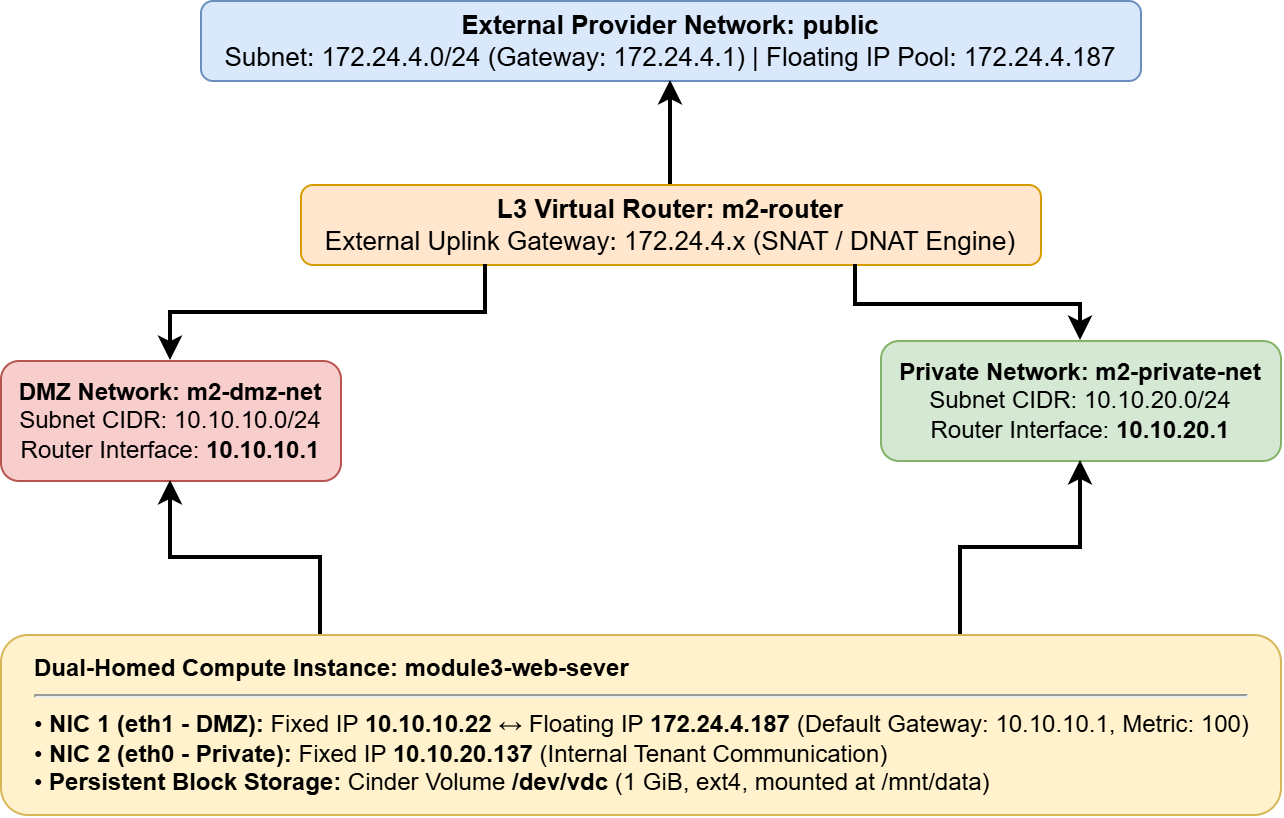
\includegraphics[width=0.92\linewidth]{img/network_topology.png}
\caption{Tô-pô mạng logic thể hiện sự cô lập đa tầng, định tuyến L3 và kết nối máy ảo đa card mạng.}
\label{fig:net_architecture}
\end{figure}

\newpage

\section{Module 1: Bảng điều khiển Horizon \& Vòng đời Dịch vụ Cốt lõi}

\subsection{Mục tiêu \& Khảo sát Ban đầu}
Trong Module 1, nhóm chúng em tiến hành kiểm tra và xác nhận trạng thái hoạt động ban đầu của toàn bộ nền tảng OpenStack ngay sau khi hoàn tất quá trình cài đặt bằng DevStack. Mục tiêu của bước này là thiết lập đường cơ sở (Baseline) tin cậy cho các lớp dịch vụ điện toán, lưu trữ và mạng, đồng thời làm quen với các thao tác quản trị trên cả giao diện đồ họa Horizon lẫn công cụ dòng lệnh OpenStack CLI.

\subsection{Kiểm tra Hiện trạng Dịch vụ Cốt lõi}
Đăng nhập vào bảng điều khiển Horizon dưới ngữ cảnh dự án \texttt{demo}, nhóm chúng em đã tiến hành khảo sát toàn diện hiện trạng của các dịch vụ:

\begin{figure}[H]
\centering
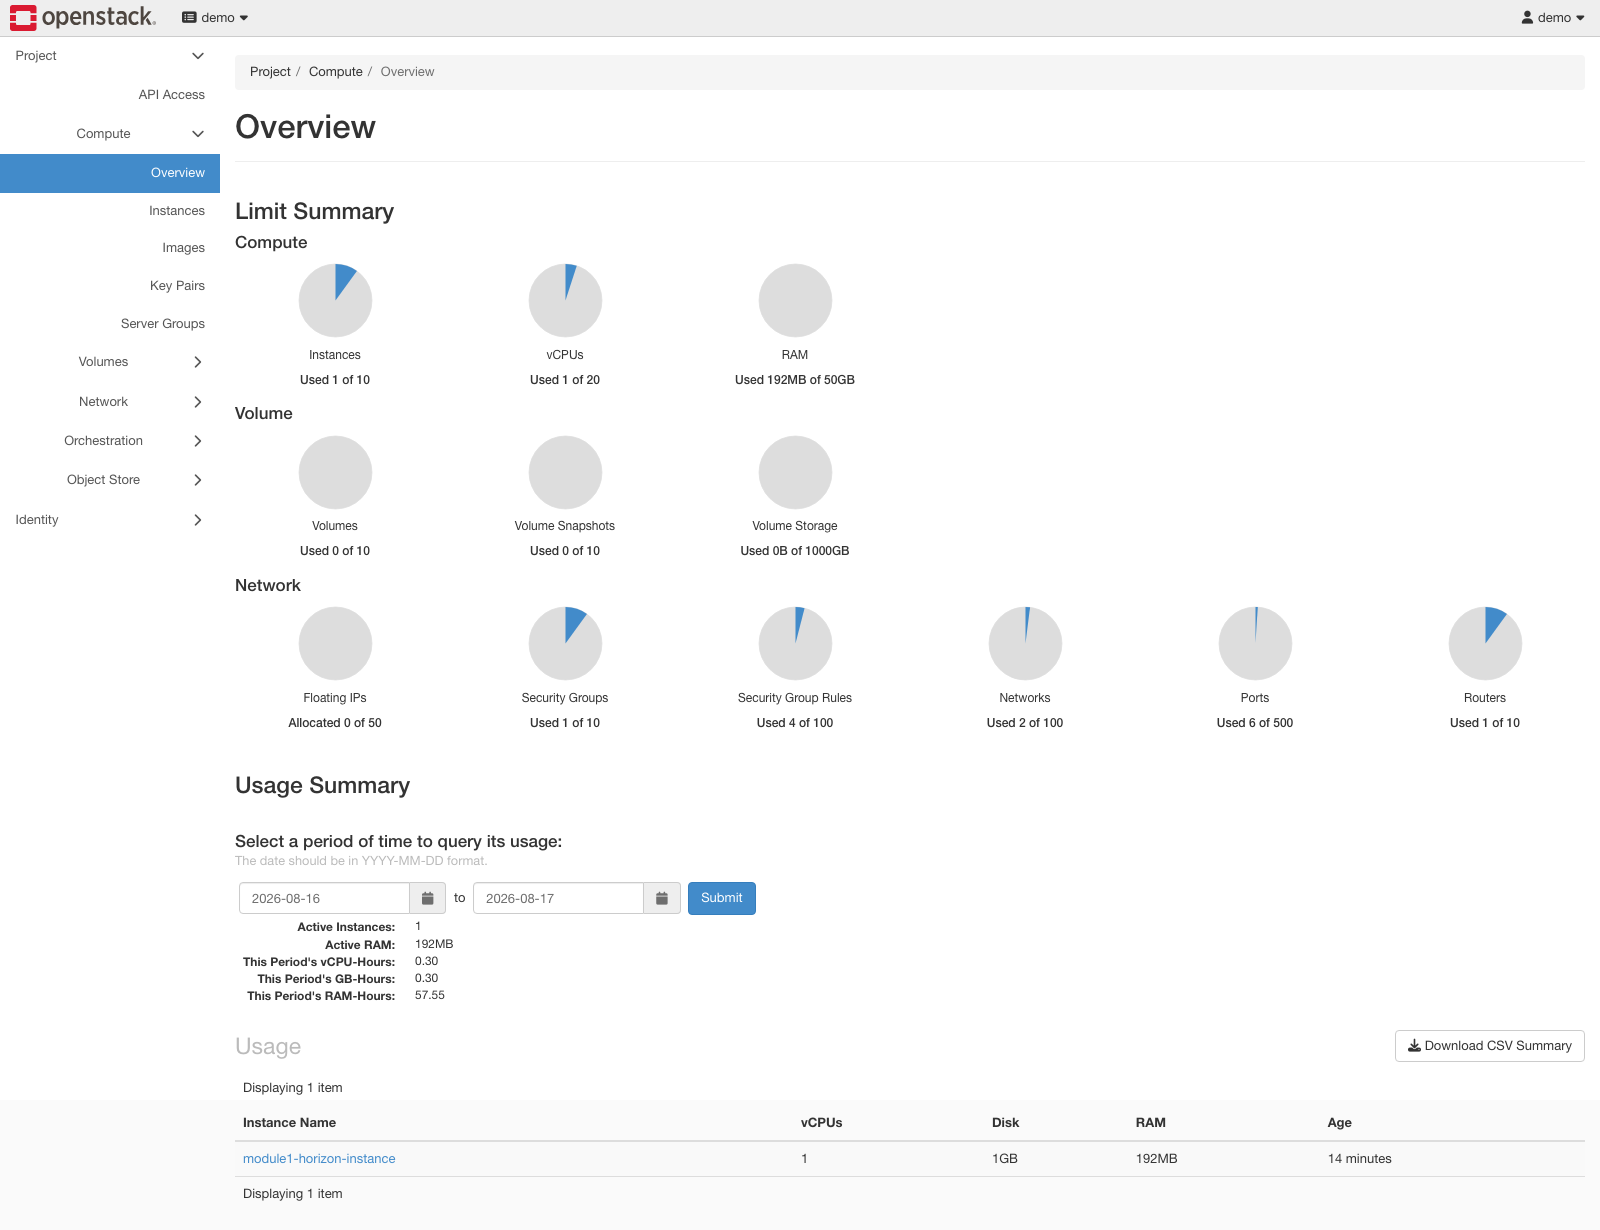
\includegraphics[width=0.88\linewidth]{img/m1-compute-resource-overview.png}
\caption{Giao diện Compute Overview và tổng quan hạn ngạch tài nguyên dự án.}
\label{fig:m1_overview}
\end{figure}

\begin{itemize}
    \item \textbf{Tổng quan Điện toán (Hình~\ref{fig:m1_overview}):} Nhóm ghi nhận hạn ngạch (Quota) mặc định của dự án gồm 10 Instances, 20 vCPUs, 50 GiB RAM, 1000 GiB Volume Storage và 50 Floating IPs.
    \item \textbf{Danh mục Ảnh máy ảo (Hình~\ref{fig:m1_glance_images}):} Dịch vụ Glance đã tích hợp sẵn hai ảnh máy ảo phục vụ thử nghiệm: bản CirrOS siêu nhẹ \nolinkurl{cirros-0.6.3-x86_64-disk} (20.69 MB) để kiểm thử nhanh và bản \nolinkurl{Fedora-Cloud-Base-37-1.7} (470 MB) cho các tác vụ Linux đầy đủ.
\end{itemize}

\begin{figure}[H]
\centering
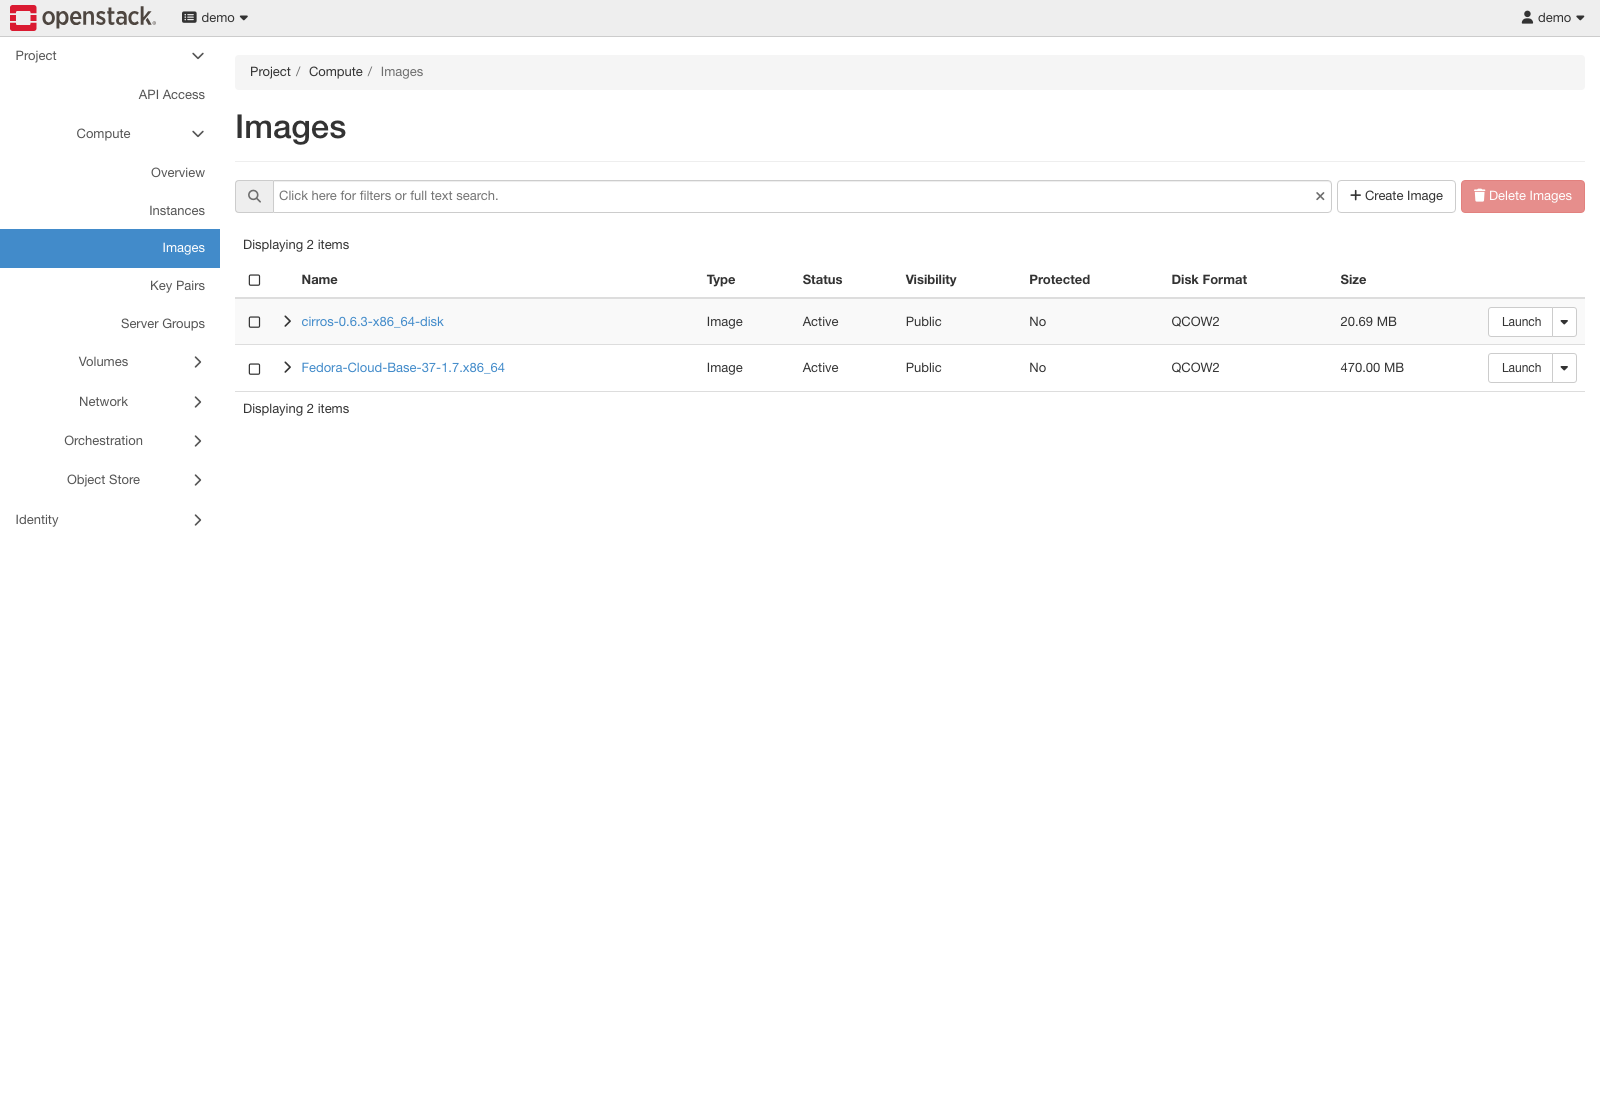
\includegraphics[width=0.88\linewidth]{img/m1-glance-image-catalog.png}
\caption{Kho lưu trữ ảnh hệ điều hành Glance đã nạp CirrOS và Fedora.}
\label{fig:m1_glance_images}
\end{figure}

\begin{itemize}
    \item \textbf{Hạ tầng Mạng ảo \& Subnet (Hình~\ref{fig:m1_networks} và~\ref{fig:m1_subnets}):} Neutron đã khởi tạo sẵn các phân đoạn mạng cơ sở gồm các mạng nội bộ tenant (\texttt{private}, \texttt{shared}, \texttt{heat-net}) và mạng ngoại vi (\texttt{public}). Phân đoạn \texttt{private-subnet} được cấu hình dual-stack hỗ trợ cả IPv4 (\nolinkurl{10.0.0.0/26}) và IPv6 (\nolinkurl{fd52:aee0:36f2::/64}).
\end{itemize}

\begin{figure}[H]
\centering
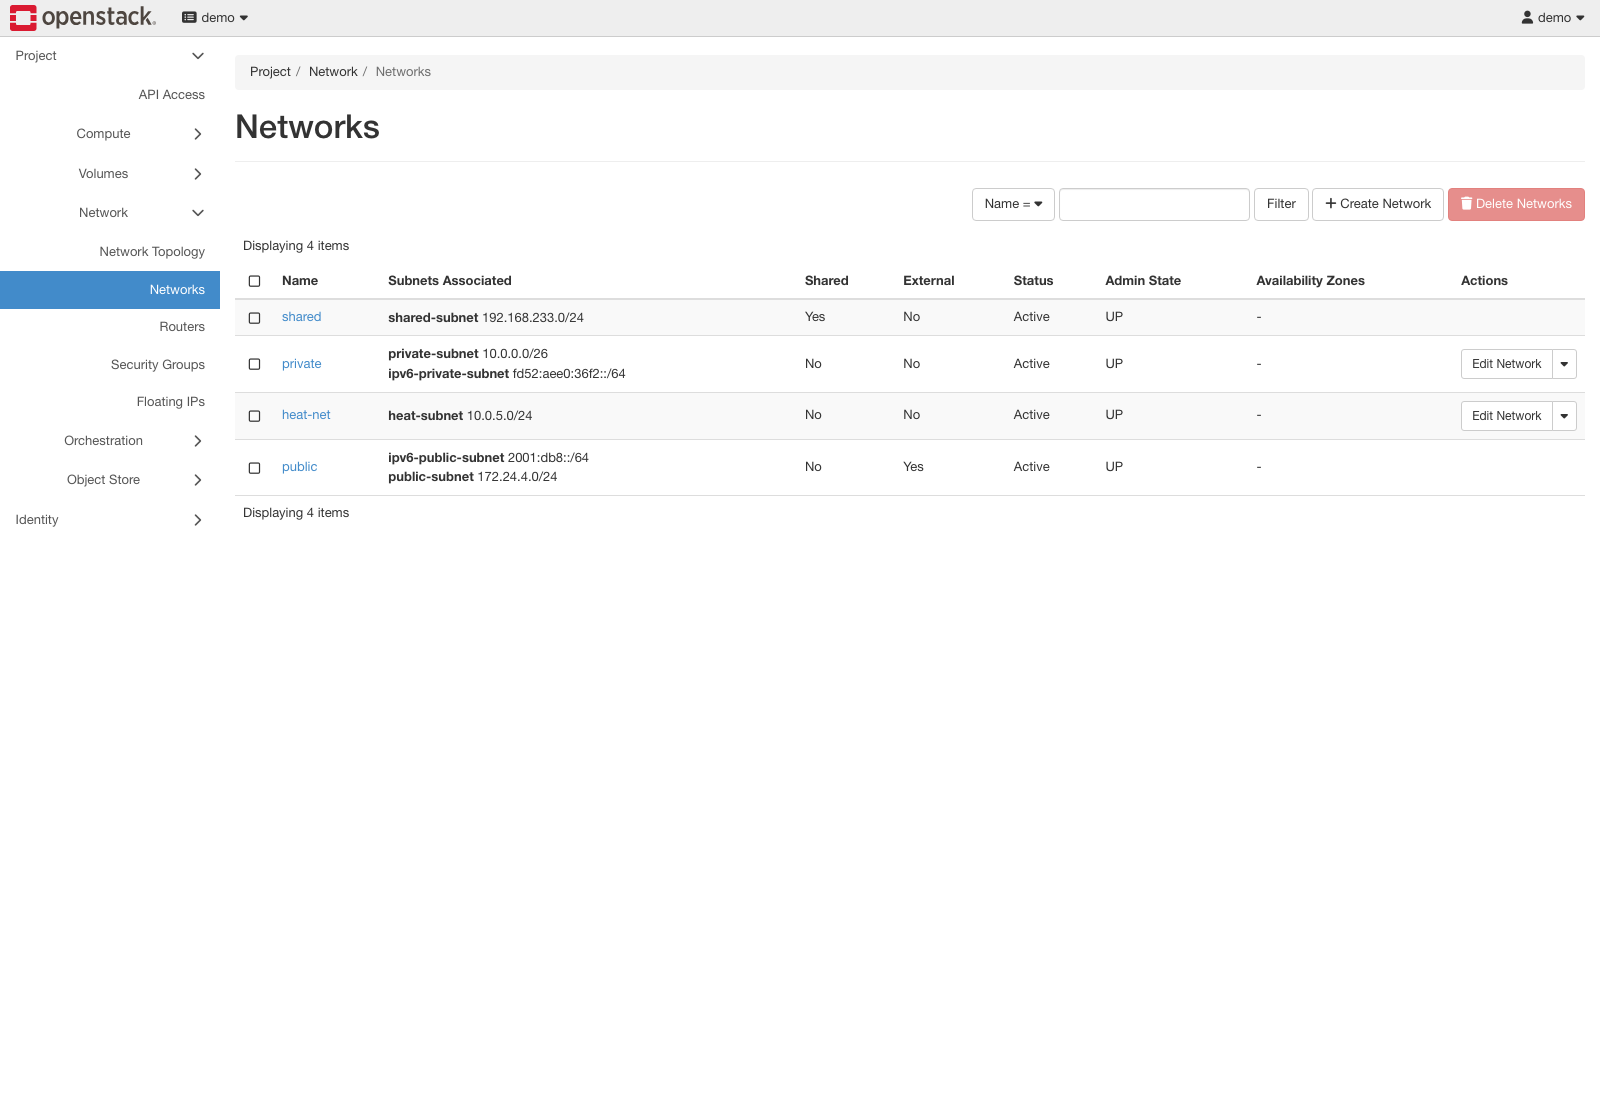
\includegraphics[width=0.88\linewidth]{img/m1-neutron-networks-list.png}
\caption{Danh sách mạng ảo hóa trong Neutron chi tiết các phân đoạn mạng.}
\label{fig:m1_networks}
\end{figure}

\begin{figure}[H]
\centering
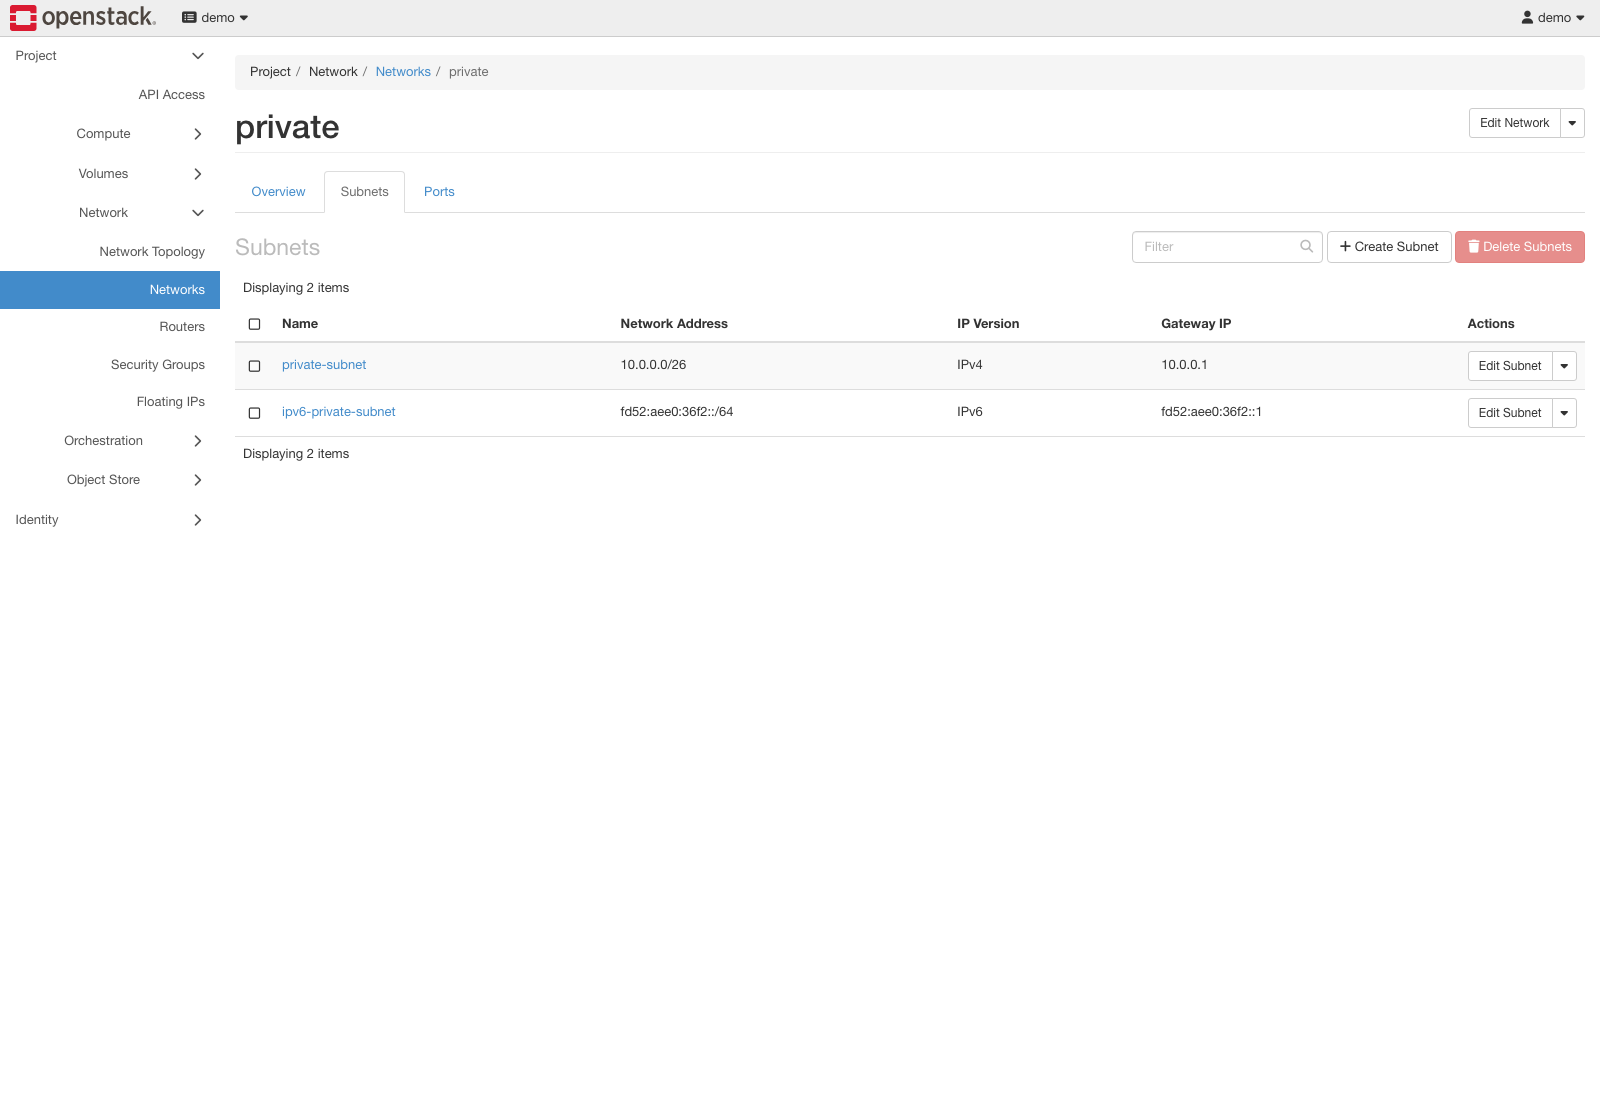
\includegraphics[width=0.88\linewidth]{img/m1-neutron-subnets-detail.png}
\caption{Chi tiết cấu hình dải địa chỉ Subnet trên mạng \texttt{private}.}
\label{fig:m1_subnets}
\end{figure}

\begin{itemize}
    \item \textbf{Bộ định tuyến L3 ảo (Hình~\ref{fig:m1_routers}):} Bộ định tuyến mặc định \texttt{router1} đang hoạt động ở trạng thái \texttt{Active}, được gắn sẵn cổng Gateway hướng ra mạng ngoài \texttt{public}.
    \item \textbf{Nhóm Bảo mật (Hình~\ref{fig:m1_secgroups}):} Nhóm tiến hành rà soát các luật tường lửa mặc định trong nhóm \texttt{default} để nắm rõ chính sách lưu lượng trước khi triển khai thêm các quy tắc mới.
\end{itemize}

\begin{figure}[H]
\centering
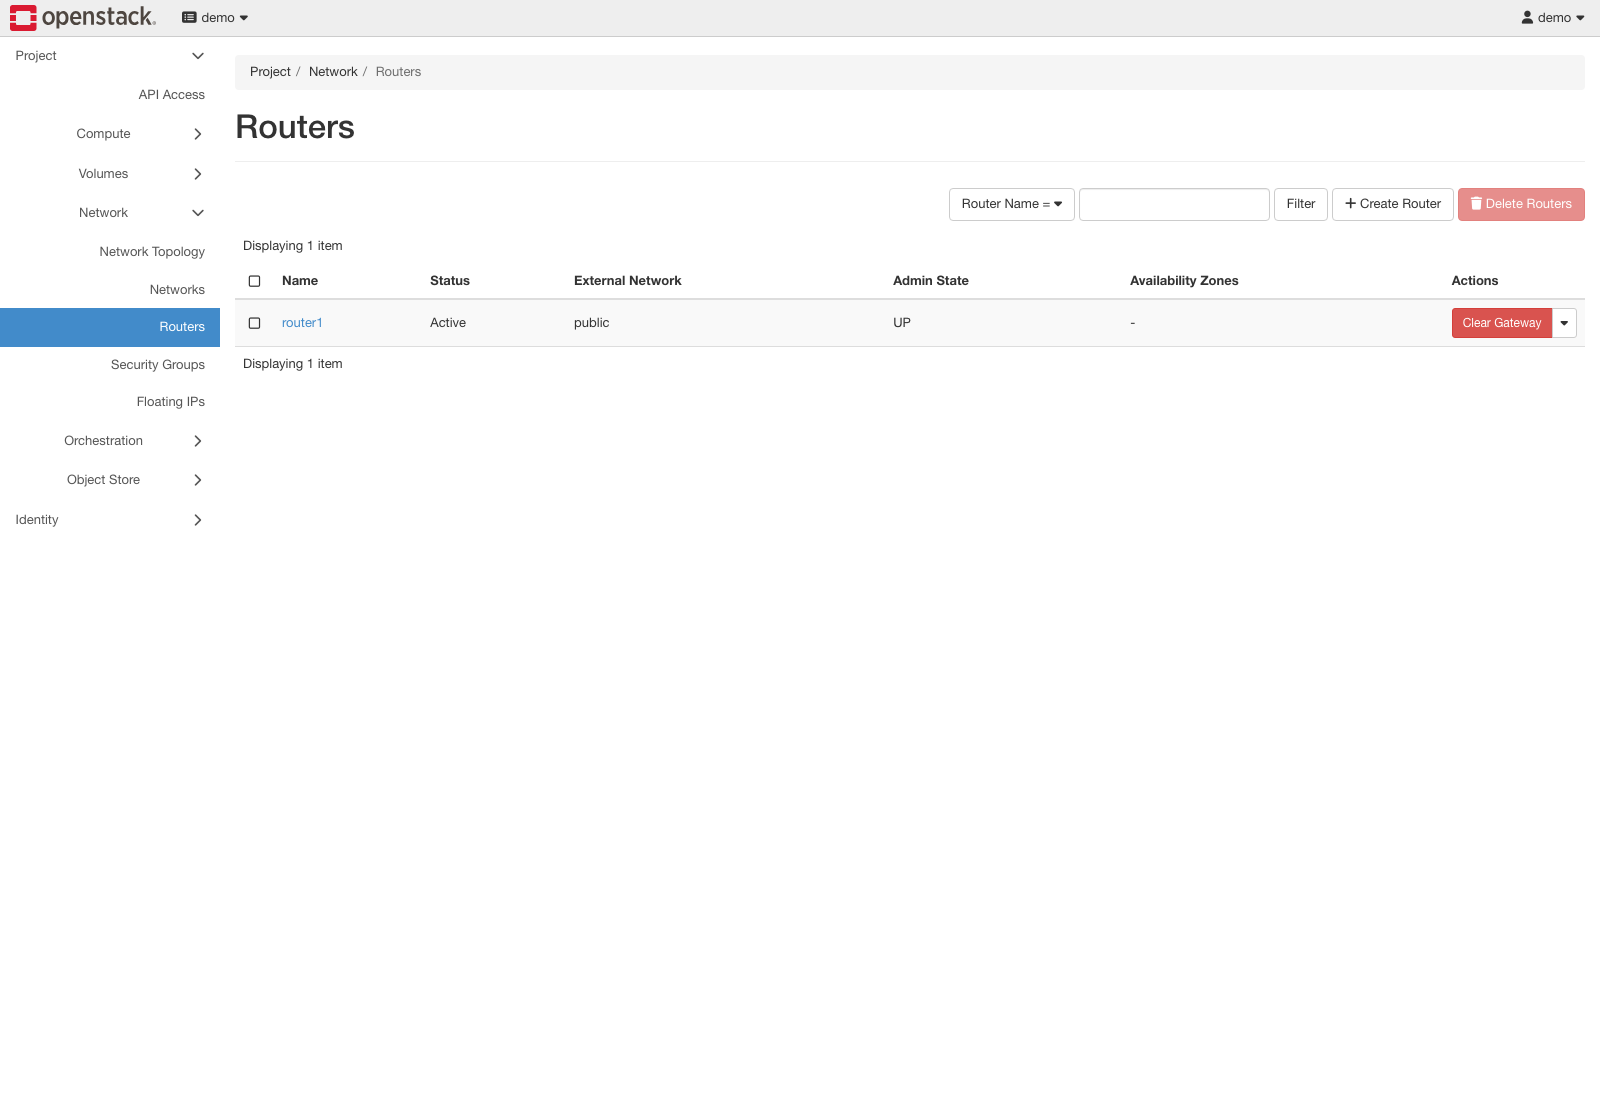
\includegraphics[width=0.88\linewidth]{img/m1-neutron-router-overview.png}
\caption{Bộ định tuyến \texttt{router1} kết nối Gateway ngoại vi ra mạng \texttt{public}.}
\label{fig:m1_routers}
\end{figure}

\begin{figure}[H]
\centering
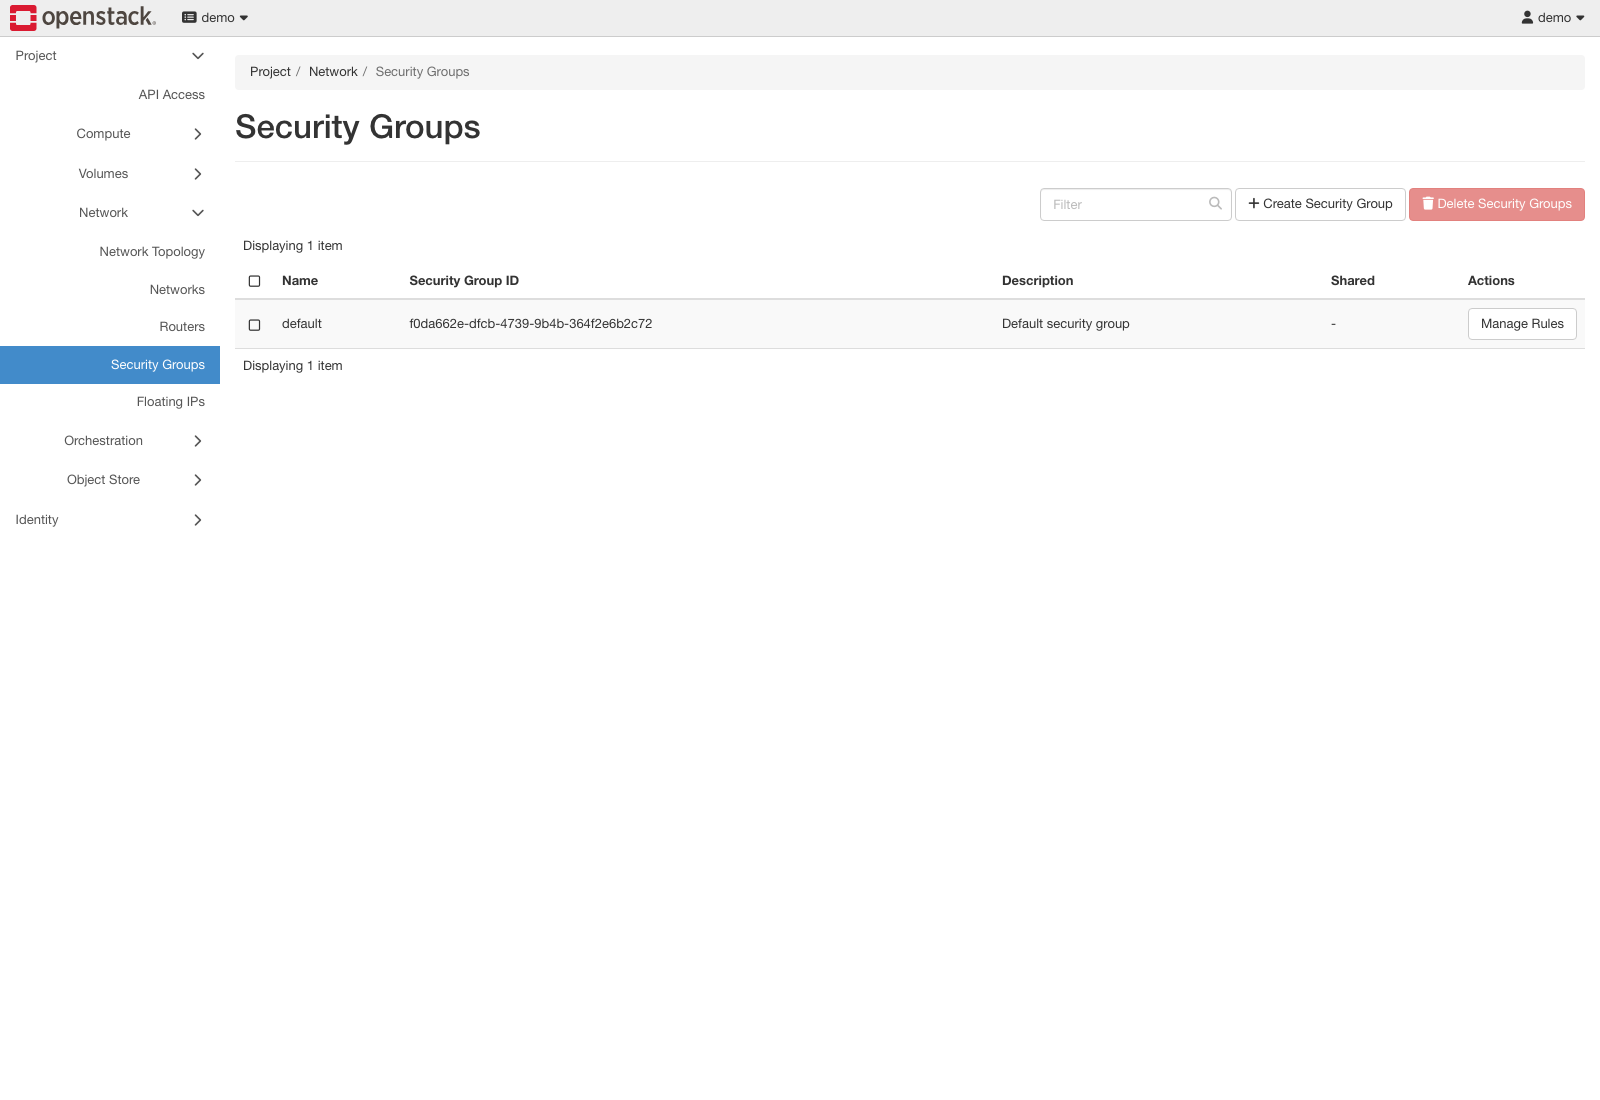
\includegraphics[width=0.88\linewidth]{img/m1-neutron-security-groups.png}
\caption{Bảng luật tường lửa Security Groups mặc định của dự án.}
\label{fig:m1_secgroups}
\end{figure}

\begin{itemize}
    \item \textbf{Khóa SSH \& Heat Stacks (Hình~\ref{fig:m1_keypairs} và~\ref{fig:m1_heat_stacks}):} Khảo sát danh mục SSH Keypair cũng như trạng thái ban đầu của bảng quản lý Heat Orchestration Stacks trước khi nạp template.
    \item \textbf{Lưu trữ Đối tượng Swift (Hình~\ref{fig:m1_swift_containers}):} Xác nhận dịch vụ Swift Object Storage đã sẵn sàng tiếp nhận yêu cầu tạo container và lưu trữ dữ liệu.
\end{itemize}

\begin{figure}[H]
\centering
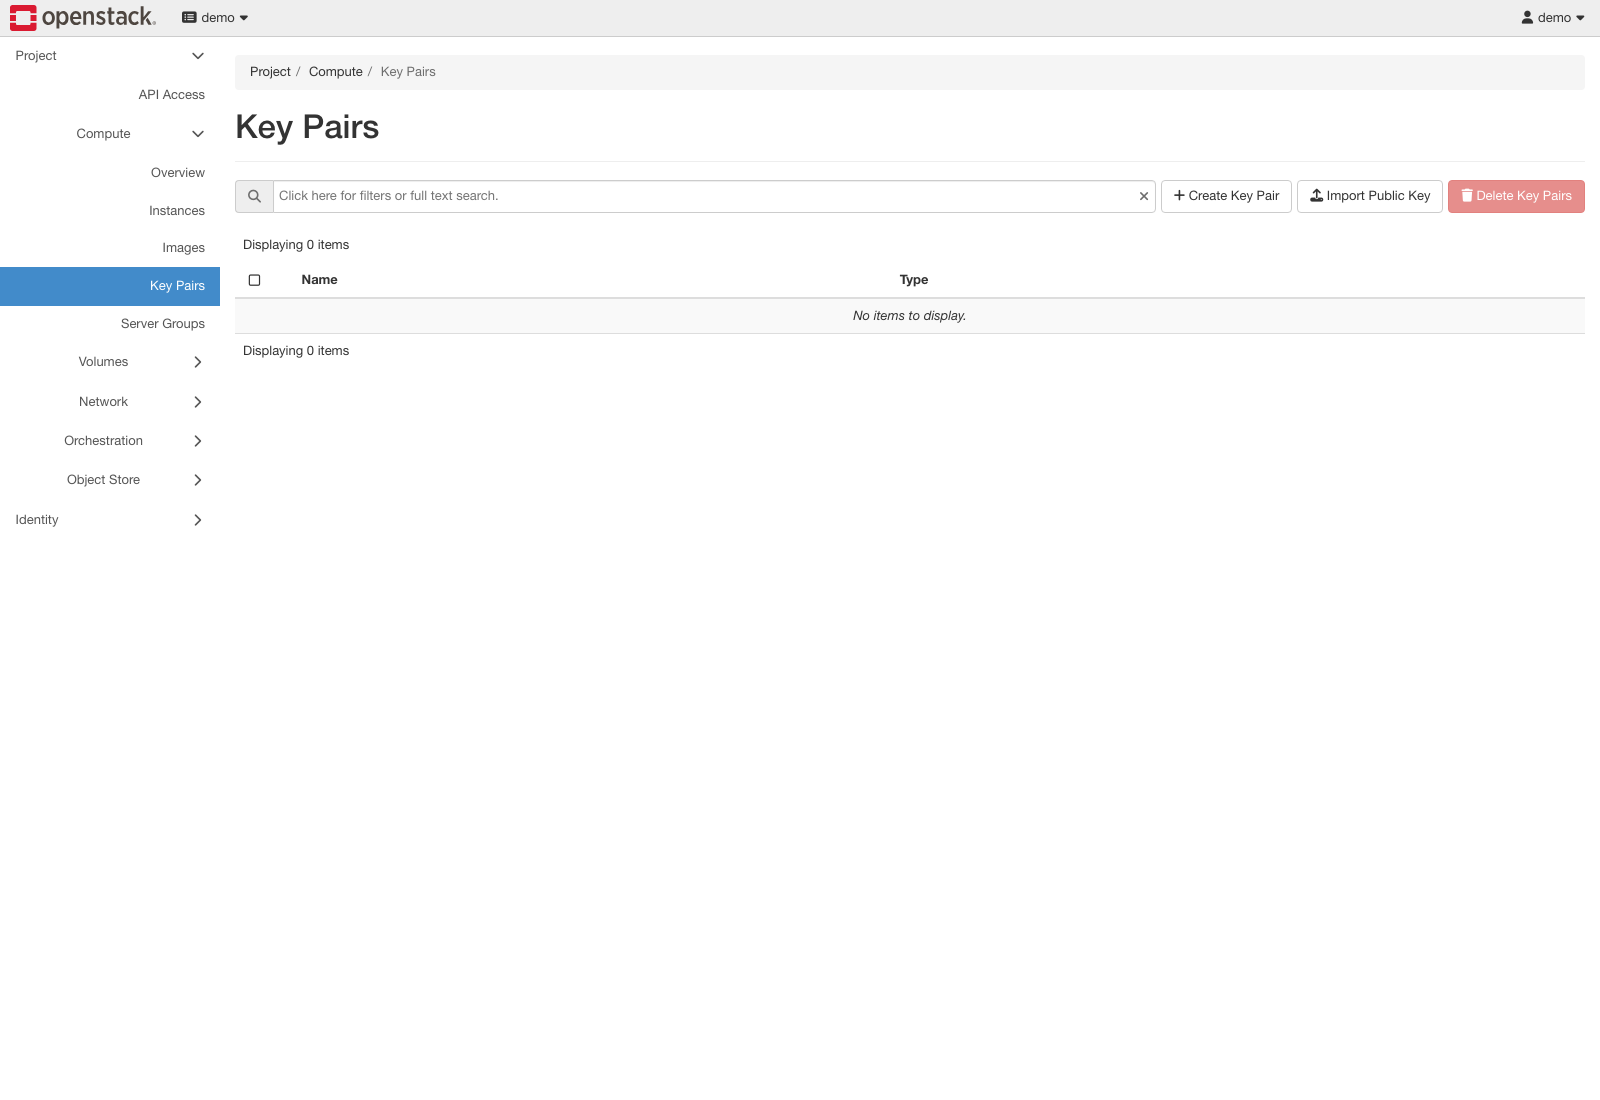
\includegraphics[width=0.88\linewidth]{img/m1-nova-keypairs-list.png}
\caption{Giao diện quản lý SSH Key Pairs trong Nova Compute.}
\label{fig:m1_keypairs}
\end{figure}

\begin{figure}[H]
\centering
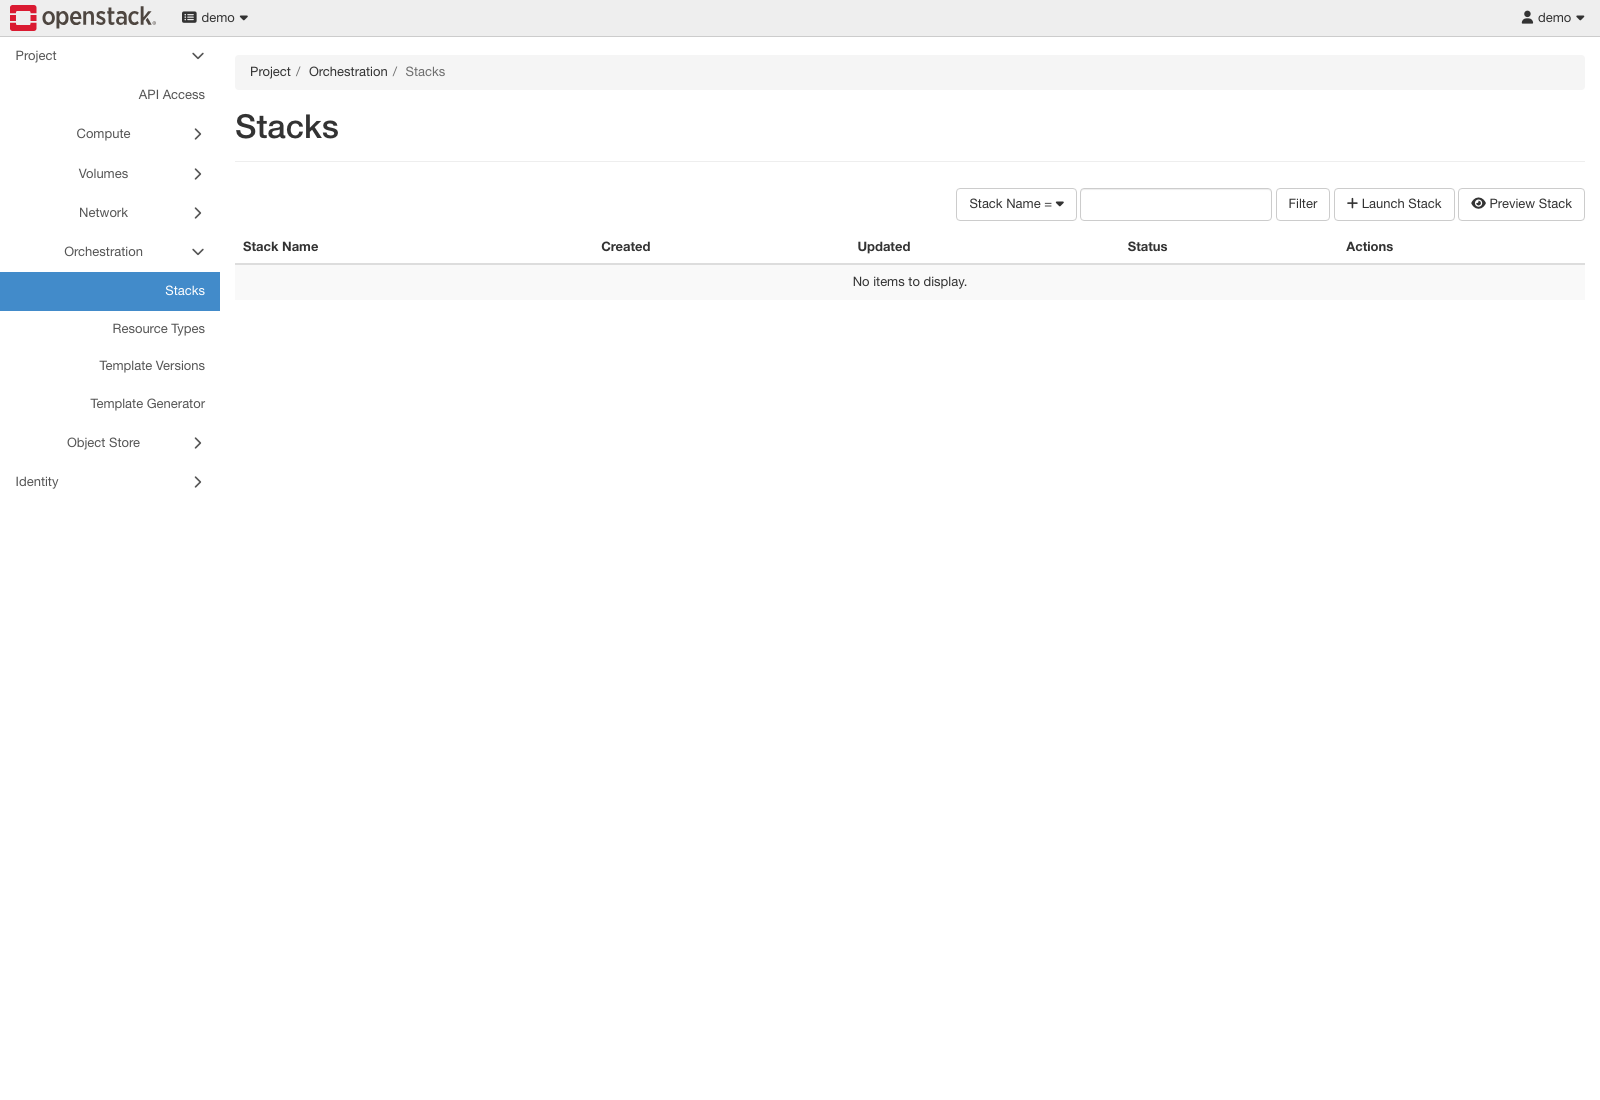
\includegraphics[width=0.88\linewidth]{img/m1-heat-stacks-initial.png}
\caption{Bảng điều khiển Heat Orchestration Stacks ở trạng thái ban đầu.}
\label{fig:m1_heat_stacks}
\end{figure}

\begin{figure}[H]
\centering
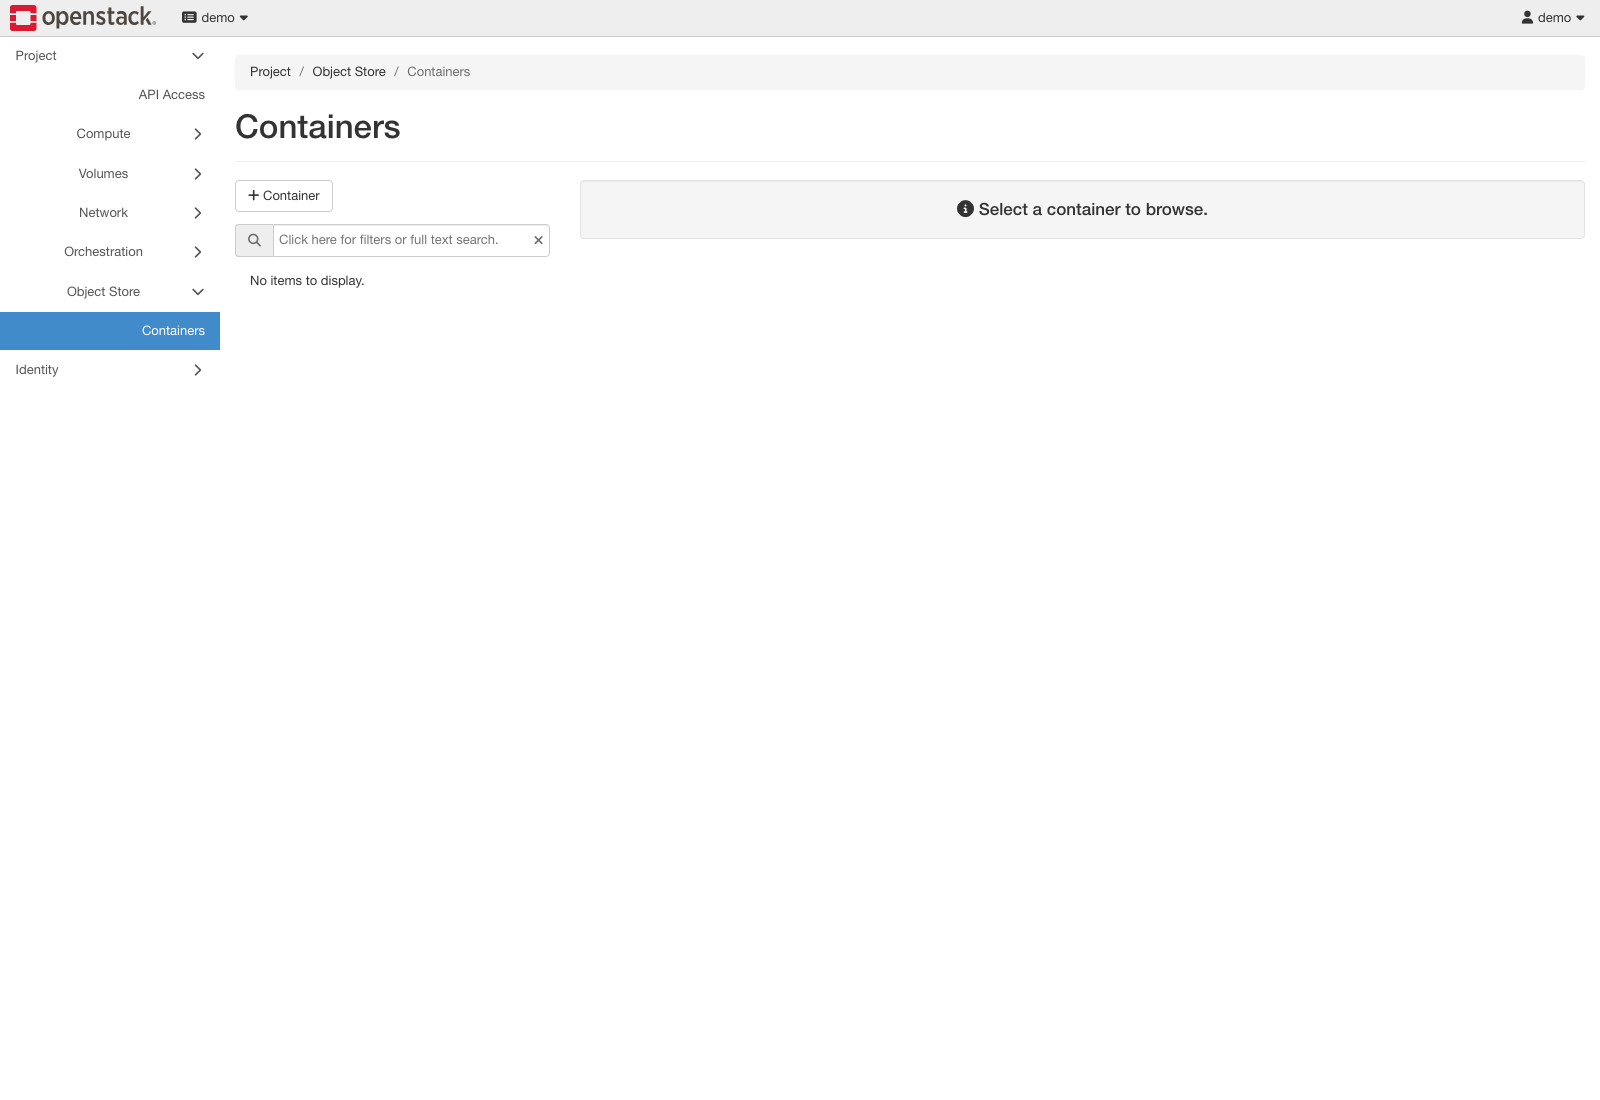
\includegraphics[width=0.88\linewidth]{img/m1-swift-containers-initial.png}
\caption{Bảng điều khiển Swift Object Storage trước khi khởi tạo vùng lưu trữ.}
\label{fig:m1_swift_containers}
\end{figure}

\subsection{Vòng đời Máy ảo: Khởi tạo, Kiểm tra Runtime \& Hủy Cấp phát}
Để kiểm chứng trọn vẹn vòng đời máy ảo cũng như quy trình lập lịch của Nova, nhóm chúng em tiến hành khởi tạo một máy ảo thử nghiệm mang tên \nolinkurl{module1-horizon-instance} thông qua wizard trên giao diện Horizon (Hình~\ref{fig:m1_launch_dialog}):
\begin{itemize}
    \item \textbf{Cấu hình khởi tạo:} Nhóm lựa chọn gói tài nguyên tối thiểu Flavor \texttt{m1.nano} (1 vCPU, 64 MB RAM, 1 GB Disk), sử dụng ảnh nguồn \nolinkurl{cirros-0.6.3-x86_64-disk} và kết nối vào mạng nội bộ \texttt{private}.
    \item \textbf{Kiểm tra trạng thái runtime (Hình~\ref{fig:m1_instance_active}):} Quá trình cấp phát diễn ra thuận lợi; máy ảo nhanh chóng chuyển sang trạng thái \texttt{Active} với Power State là \texttt{Running}, được gán địa chỉ IP nội bộ \texttt{10.0.0.45} (IPv4) và \nolinkurl{fd52:aee0:36f2:0:f816:3eff:fed0:3caa} (IPv6).
    \item \textbf{Hủy cấp phát và thu hồi tài nguyên (Hình~\ref{fig:m1_delete_confirmation} và~\ref{fig:m1_instances_empty}):} Sau khi kiểm tra xong, nhóm thực hiện thao tác xóa máy ảo. Giao diện Horizon cập nhật danh sách máy ảo về trạng thái rỗng, qua đó xác nhận hệ thống đã giải phóng hoàn toàn các tài nguyên vCPU, RAM và cổng mạng ảo về lại quota chung của dự án.
\end{itemize}

\begin{figure}[H]
\centering
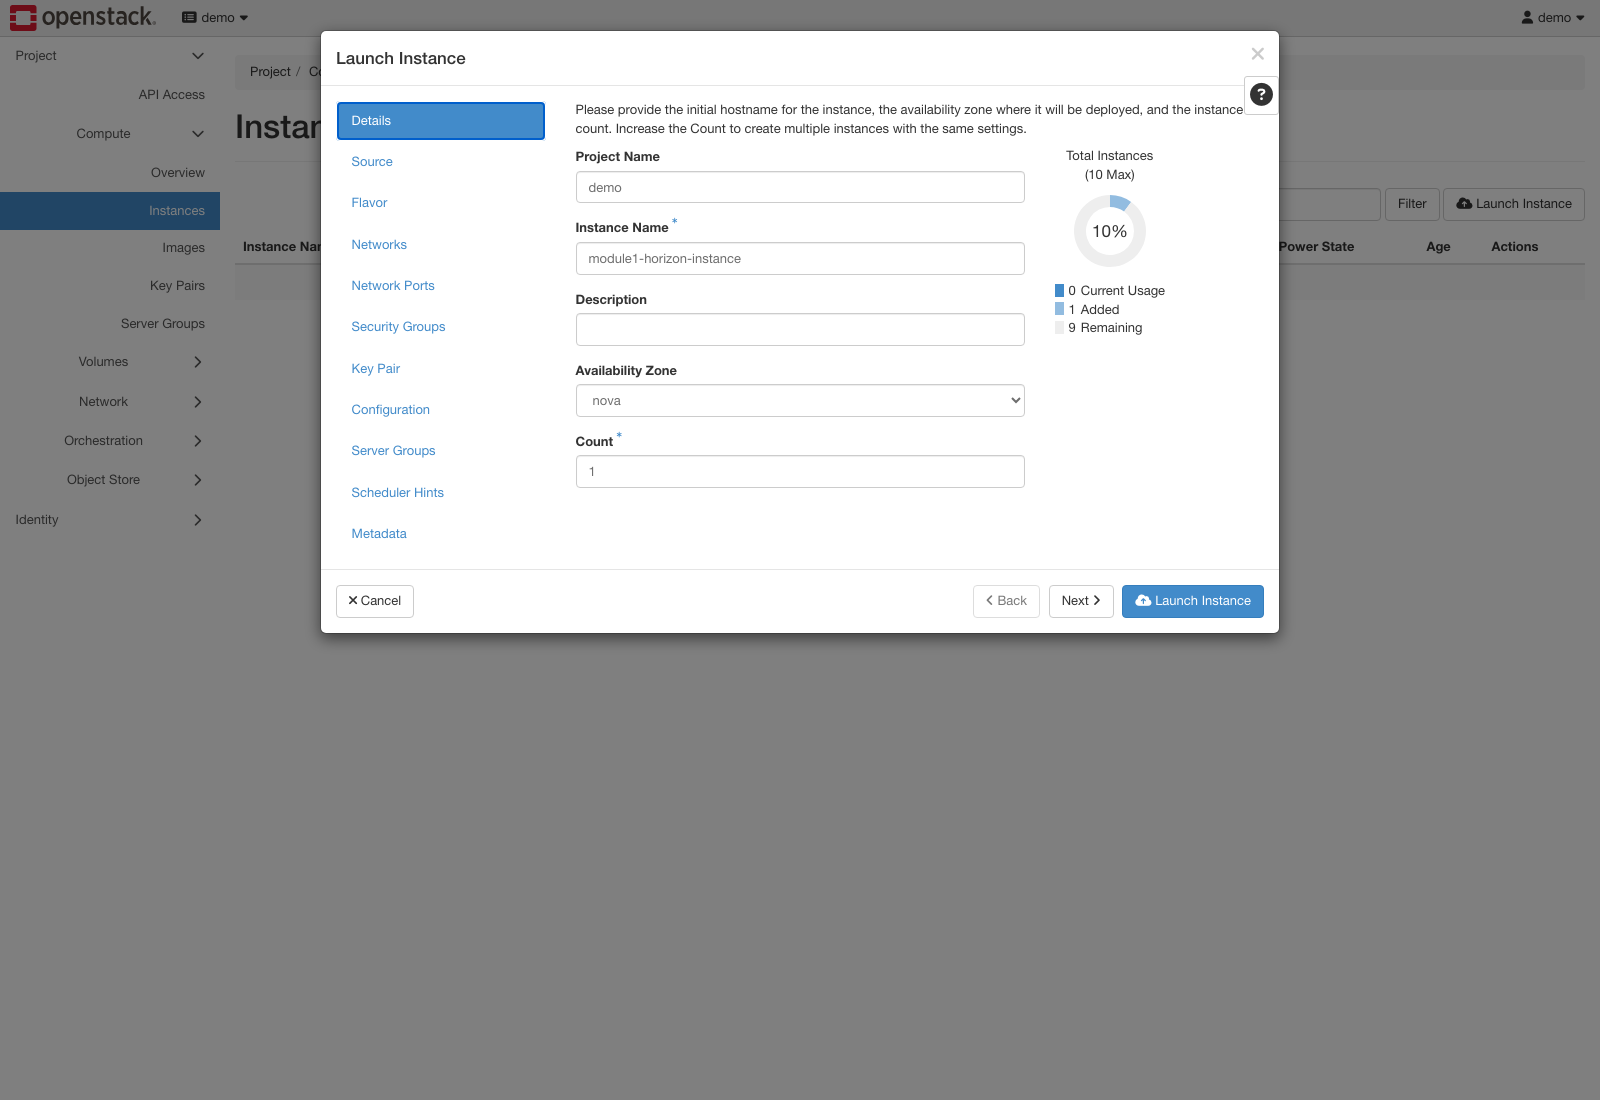
\includegraphics[width=0.88\linewidth]{img/m1-instance-launch-wizard.png}
\caption{Wizard khởi tạo máy ảo trong Horizon thể hiện các thông số cấu hình.}
\label{fig:m1_launch_dialog}
\end{figure}

\begin{figure}[H]
\centering
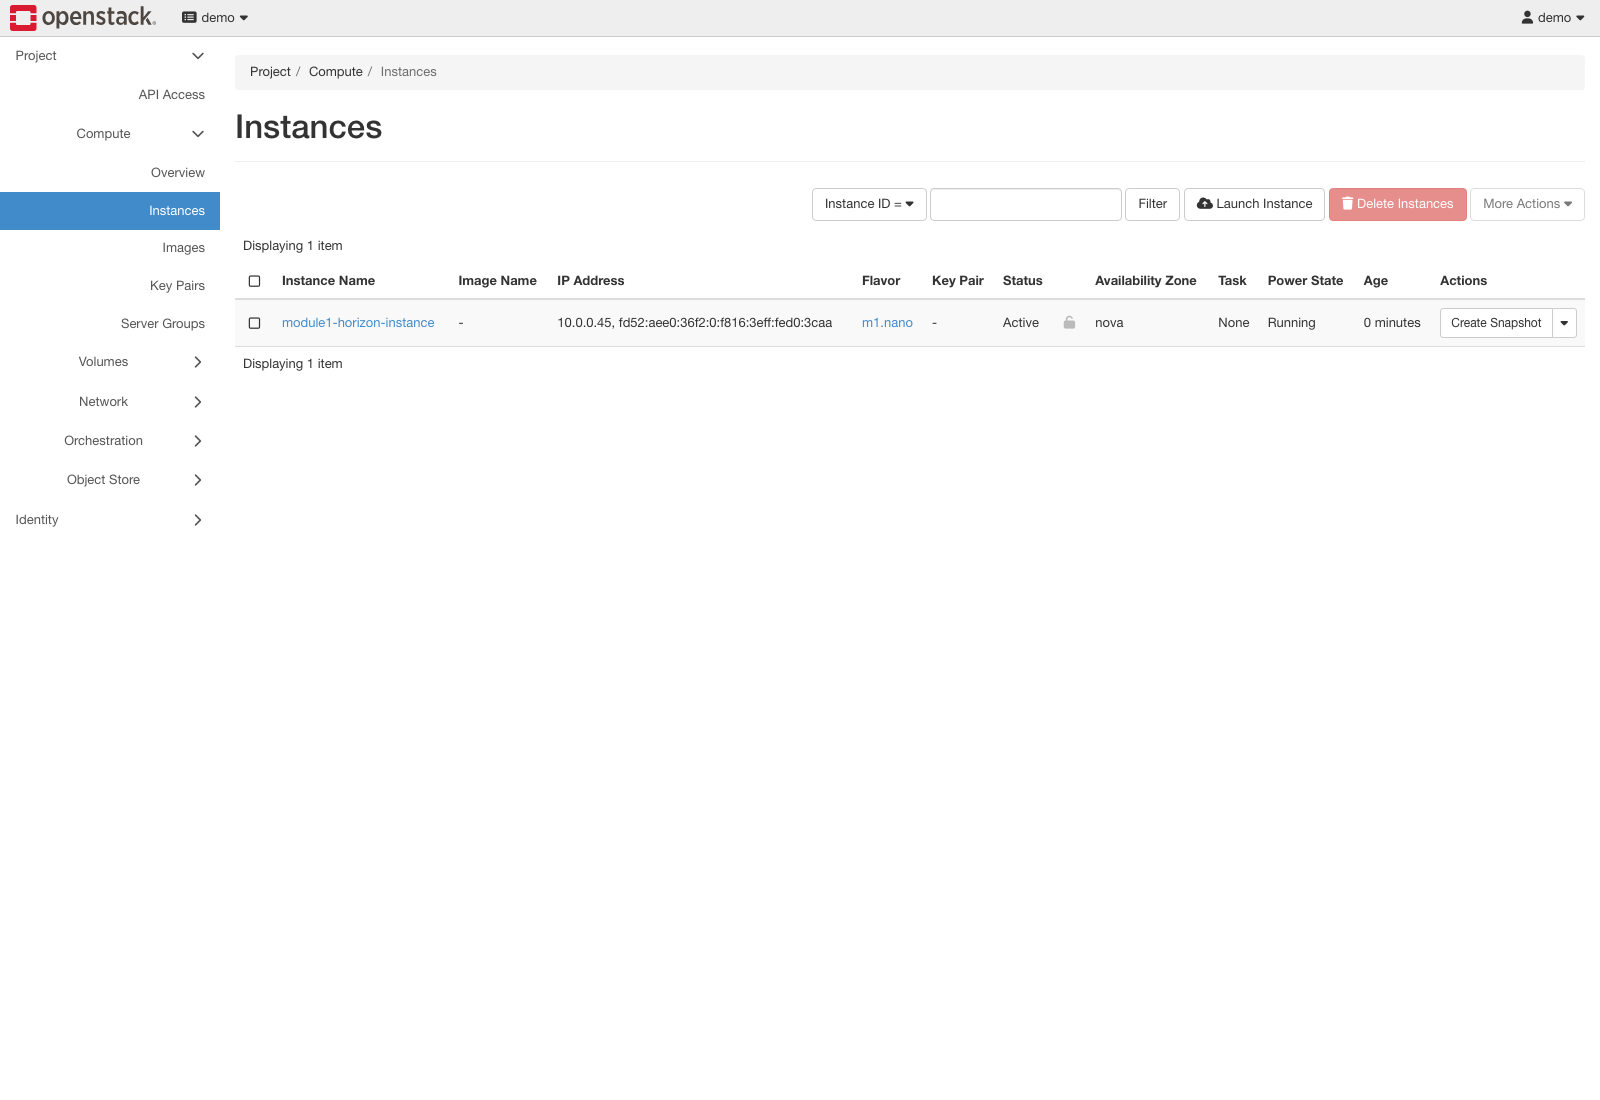
\includegraphics[width=0.88\linewidth]{img/m1-instance-active-status.png}
\caption{Máy ảo đạt trạng thái Active với Power State Running trong Nova.}
\label{fig:m1_instance_active}
\end{figure}

\begin{figure}[H]
\centering
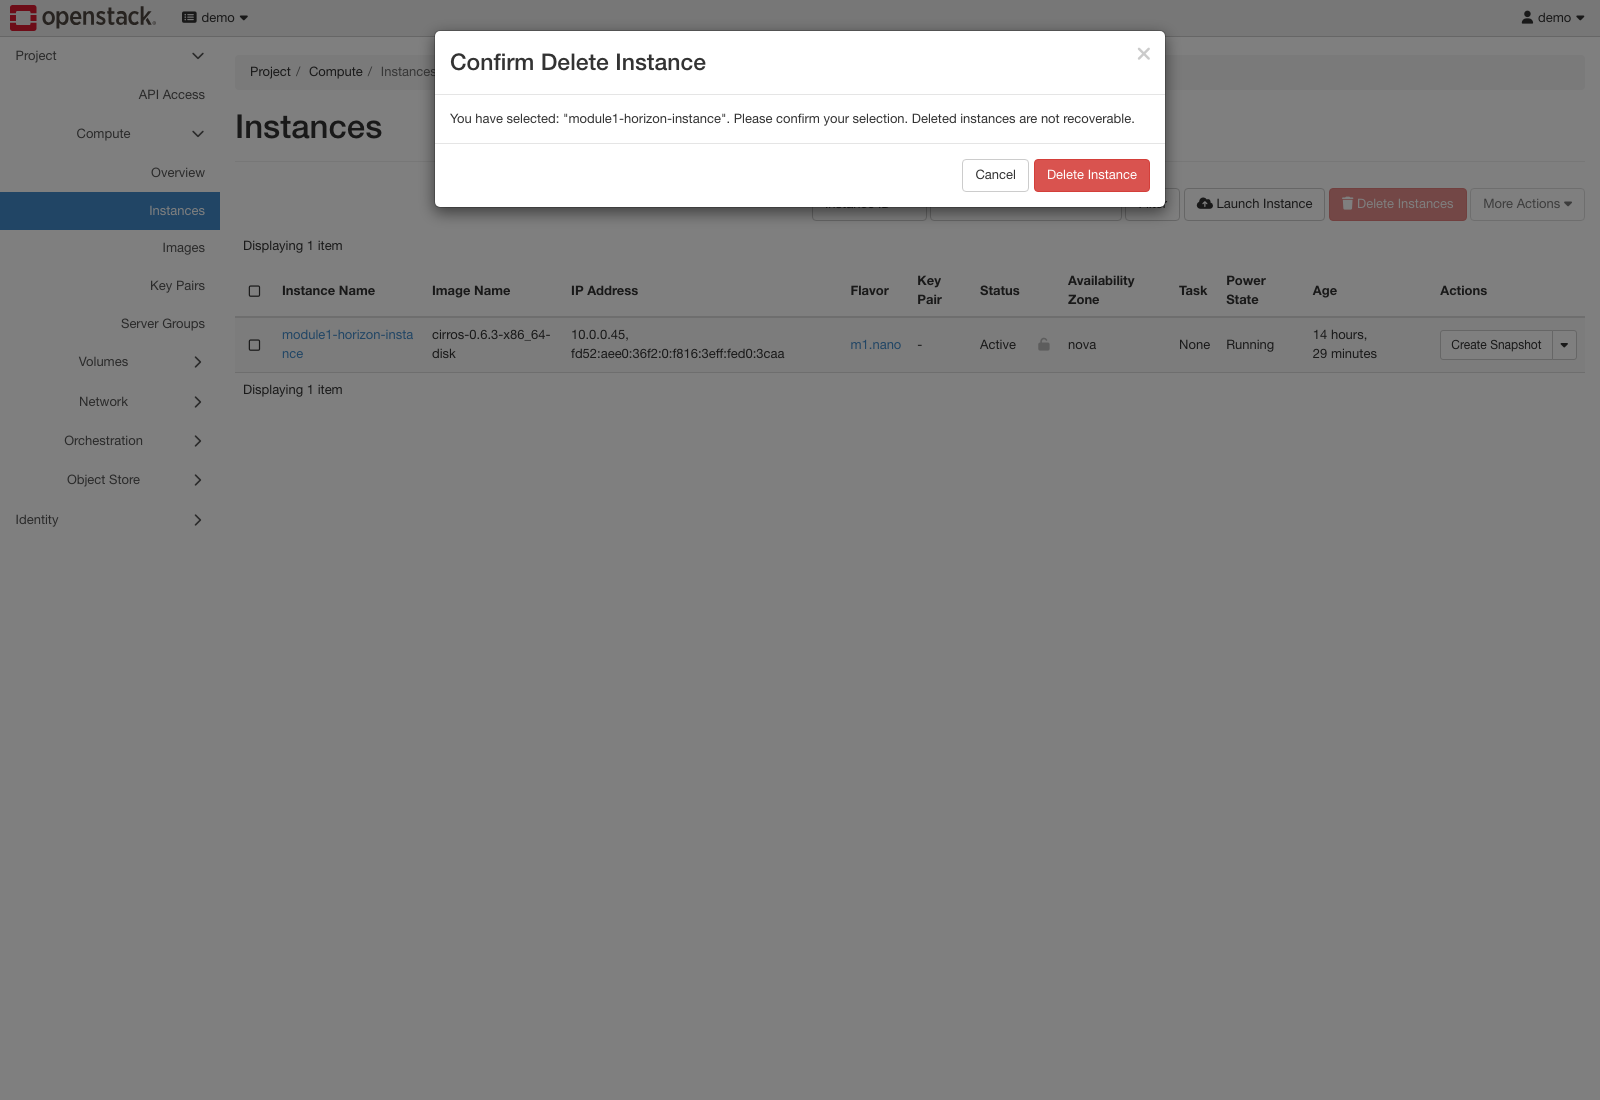
\includegraphics[width=0.88\linewidth]{img/m1-instance-delete-confirmation.png}
\caption{Modal xác nhận xóa máy ảo \nolinkurl{module1-horizon-instance}.}
\label{fig:m1_delete_confirmation}
\end{figure}

\begin{figure}[H]
\centering
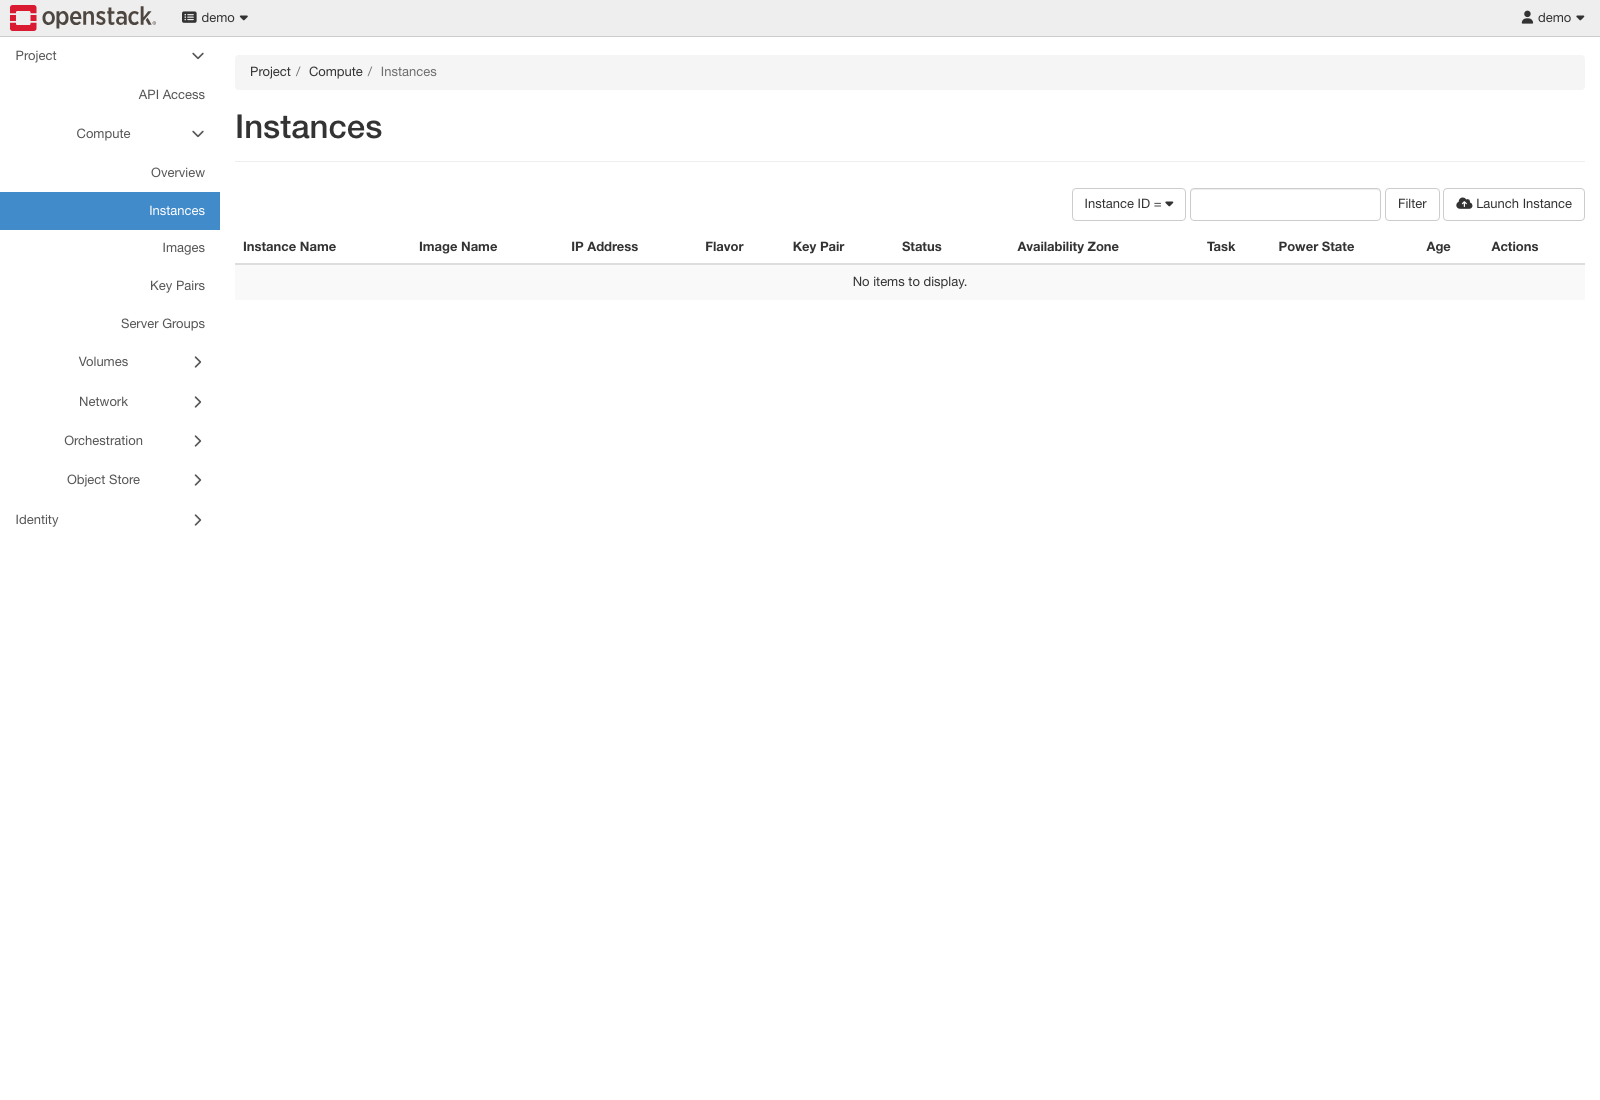
\includegraphics[width=0.88\linewidth]{img/m1-instance-terminated-empty.png}
\caption{Danh sách máy ảo rỗng sau khi thu hồi tài nguyên thành công.}
\label{fig:m1_instances_empty}
\end{figure}

\newpage

\section{Module 2: Cô lập Mạng Đa tầng cho Tenant}

\subsection{Mục tiêu \& Nguyên lý Thiết kế}
Trong Module 2, nhóm chúng em tiến hành xây dựng một kiến trúc mạng ảo hai tầng độc lập nhằm phân tách ranh giới an ninh giữa vùng dịch vụ tiếp nhận lưu lượng bên ngoài (DMZ) và vùng cơ sở dữ liệu/backend nội bộ (Private). Dựa trên nền tảng mạng điều khiển bằng phần mềm (Neutron SDN), nhóm thiết lập các miền quảng bá (Broadcast Domains) riêng biệt kèm theo chính sách định tuyến tầng 3 (L3 Routing) linh hoạt, giúp kiểm soát chặt chẽ luồng thông tin giữa các phân vùng.

\subsection{Quy trình Cấu hình Thực tế}
Quá trình thiết lập hạ tầng mạng được nhóm chúng em triển khai tuần tự theo 4 bước kỹ thuật sau:

\begin{enumerate}
    \item \textbf{Khởi tạo Mạng DMZ \& Subnet:}
    \begin{itemize}
        \item Tên mạng: \texttt{m2-dmz-net} (\texttt{module2-dmz-net})
        \item Dải Subnet: \texttt{10.10.10.0/24}, Gateway IP: \texttt{10.10.10.1}, DNS: \texttt{8.8.8.8}
    \end{itemize}
    \item \textbf{Khởi tạo Mạng Nội bộ Private \& Subnet:}
    \begin{itemize}
        \item Tên mạng: \texttt{m2-private-net} (\texttt{module2-private-net})
        \item Dải Subnet: \texttt{10.10.20.0/24}, Gateway IP: \texttt{10.10.20.1}, DNS: \texttt{8.8.8.8}
    \end{itemize}
    \item \textbf{Khởi tạo Bộ định tuyến L3 Router \& Cổng Gateway Ngoại vi:}
    \begin{itemize}
        \item Tên Router: \texttt{m2-router} (\texttt{module2-router})
        \item External Gateway: Gắn trực tiếp vào mạng nhà cung cấp ngoài \texttt{public} để kích hoạt tính năng chuyển đổi địa chỉ mạng nguồn (SNAT) và cho phép ánh xạ Floating IP sau này.
    \end{itemize}
    \item \textbf{Đính kèm Giao diện Mạng vào Router (Router Interfaces):}
    Gắn lần lượt hai cổng giao diện \texttt{m2-dmz-subnet} và \texttt{m2-private-subnet} vào \texttt{m2-router}. Thao tác này kích hoạt chức năng định tuyến liên mạng con (Inter-Subnet Routing) giữa vùng DMZ và Private nhưng vẫn bảo đảm sự cô lập tầng 2 (L2 Isolation).
\end{enumerate}

\subsection{Kiểm tra \& Phân tích Tô-pô Mạng}
Sau khi hoàn tất cấu hình, nhóm chúng em tiến hành nghiệm thu và phân tích hiện trạng tô-pô mạng thông qua cả giao diện Horizon lẫn OpenStack CLI:

\begin{figure}[H]
\centering
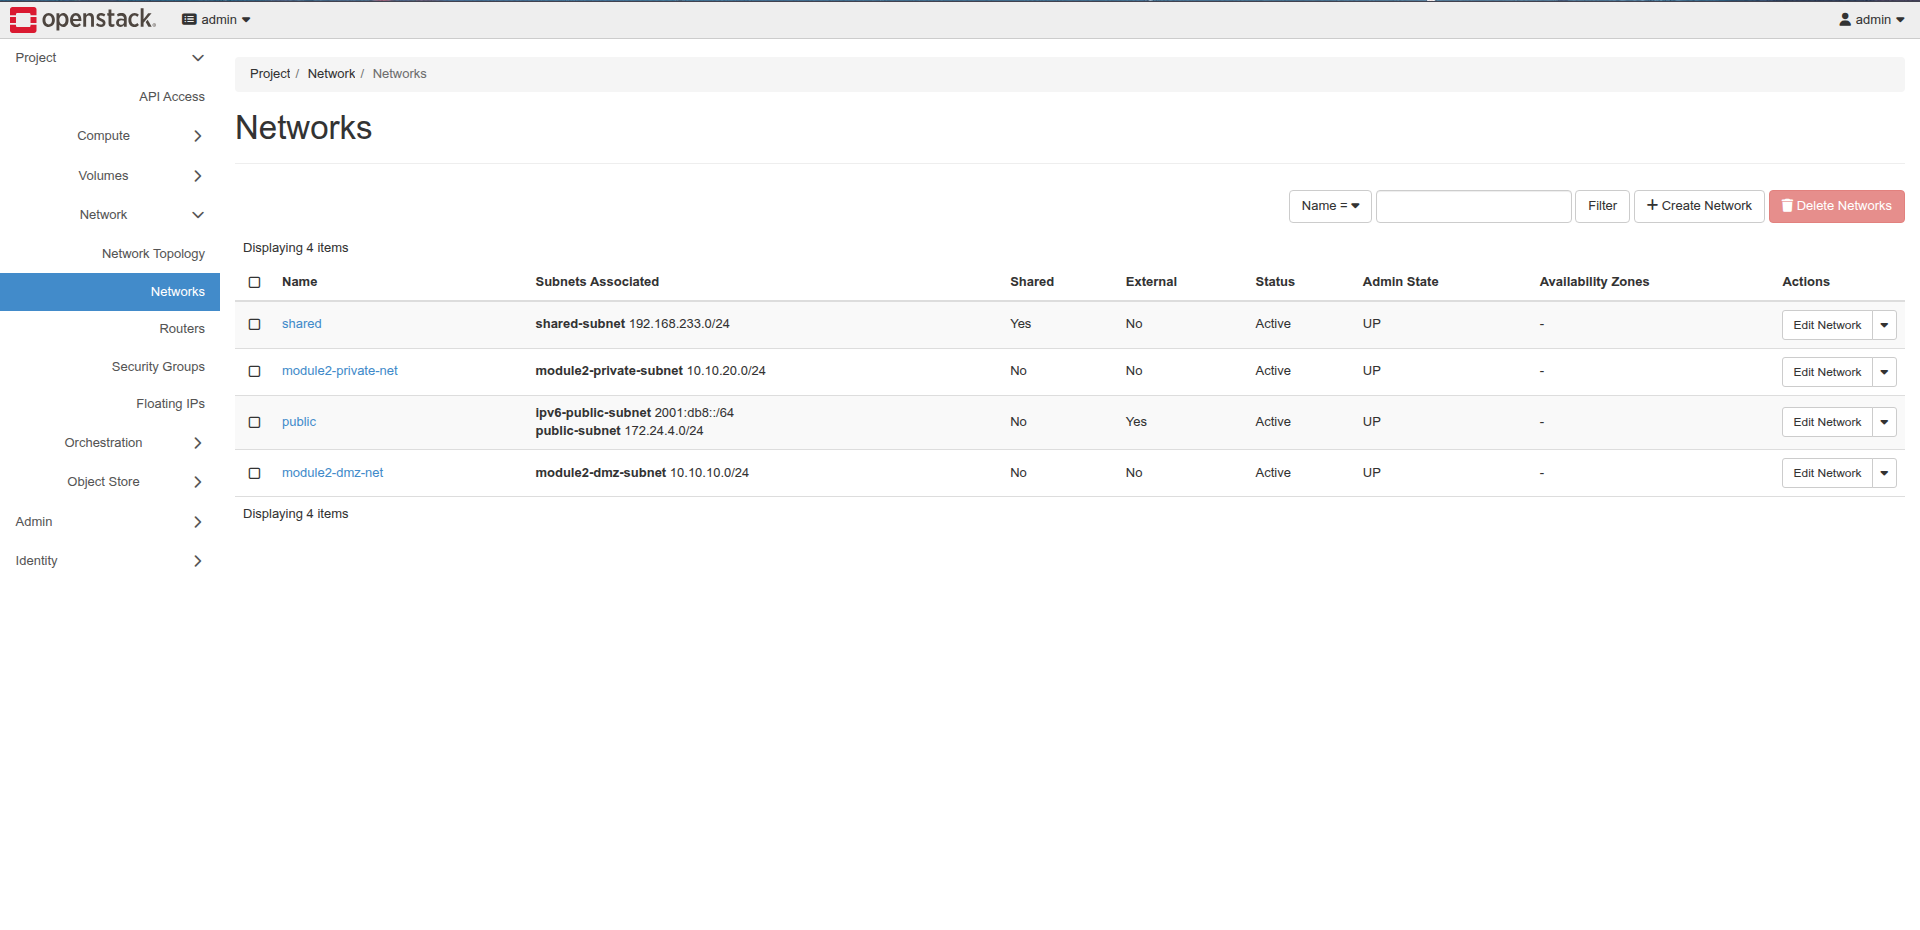
\includegraphics[width=0.88\linewidth]{img/m2-network-list.png}
\caption{Danh sách mạng Neutron hiển thị hai subnet DMZ và Private vừa tạo.}
\label{fig:m2_networks}
\end{figure}

\begin{itemize}
    \item \textbf{Trạng thái các Subnet (Hình~\ref{fig:m2_networks}):} Cả hai subnet tenant (\nolinkurl{10.10.10.0/24} và \nolinkurl{10.10.20.0/24}) đều đã khởi tạo thành công và ở trạng thái sẵn sàng hoạt động.
    \item \textbf{Cổng External Gateway của Router (Hình~\ref{fig:m2_router_overview}):} Nhóm xác nhận bộ định tuyến \texttt{module2-router} đã nhận địa chỉ IP ngoại vi thuộc mạng \texttt{public}, sẵn sàng làm cầu nối ra bên ngoài.
    \item \textbf{Cổng Giao diện Nội bộ (Hình~\ref{fig:m2_router_interfaces}):} Xác nhận \texttt{module2-router} đã liên kết thành công 2 cổng nội bộ đóng vai trò Default Gateway tương ứng cho DMZ (\texttt{10.10.10.1}) và Private (\texttt{10.10.20.1}).
\end{itemize}

\begin{figure}[H]
\centering
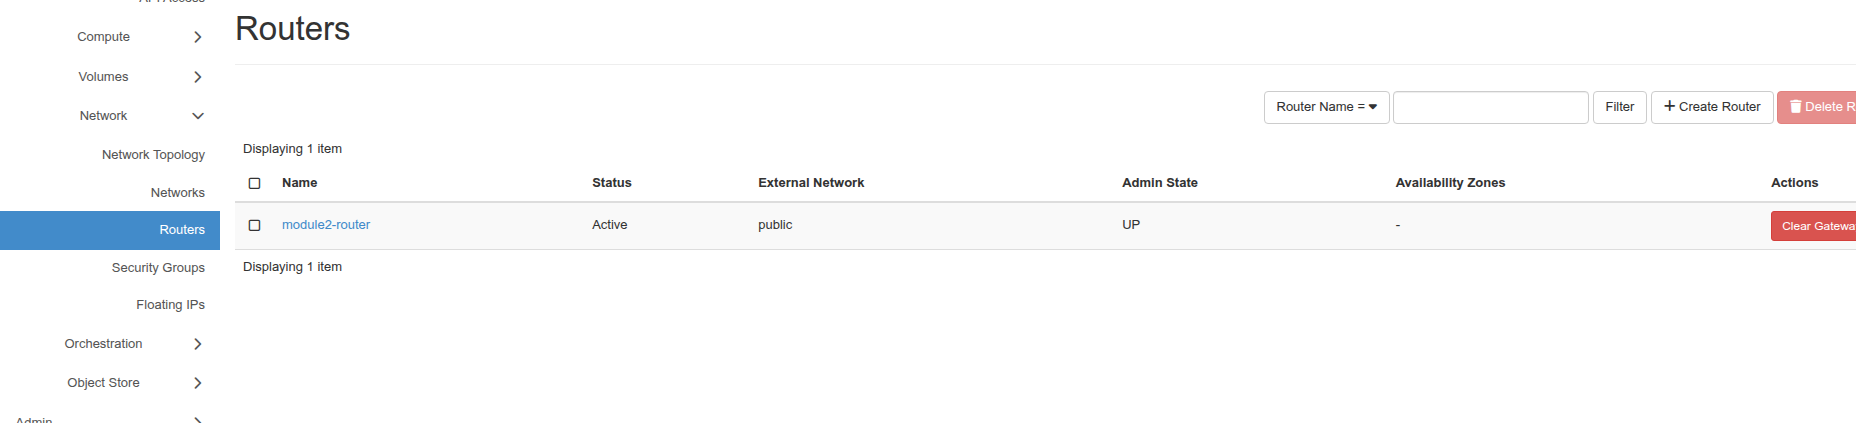
\includegraphics[width=0.88\linewidth]{img/m2-router-external-gateway.png}
\caption{Bộ định tuyến \texttt{module2-router} kết nối uplink ra mạng \texttt{public}.}
\label{fig:m2_router_overview}
\end{figure}

\begin{figure}[H]
\centering
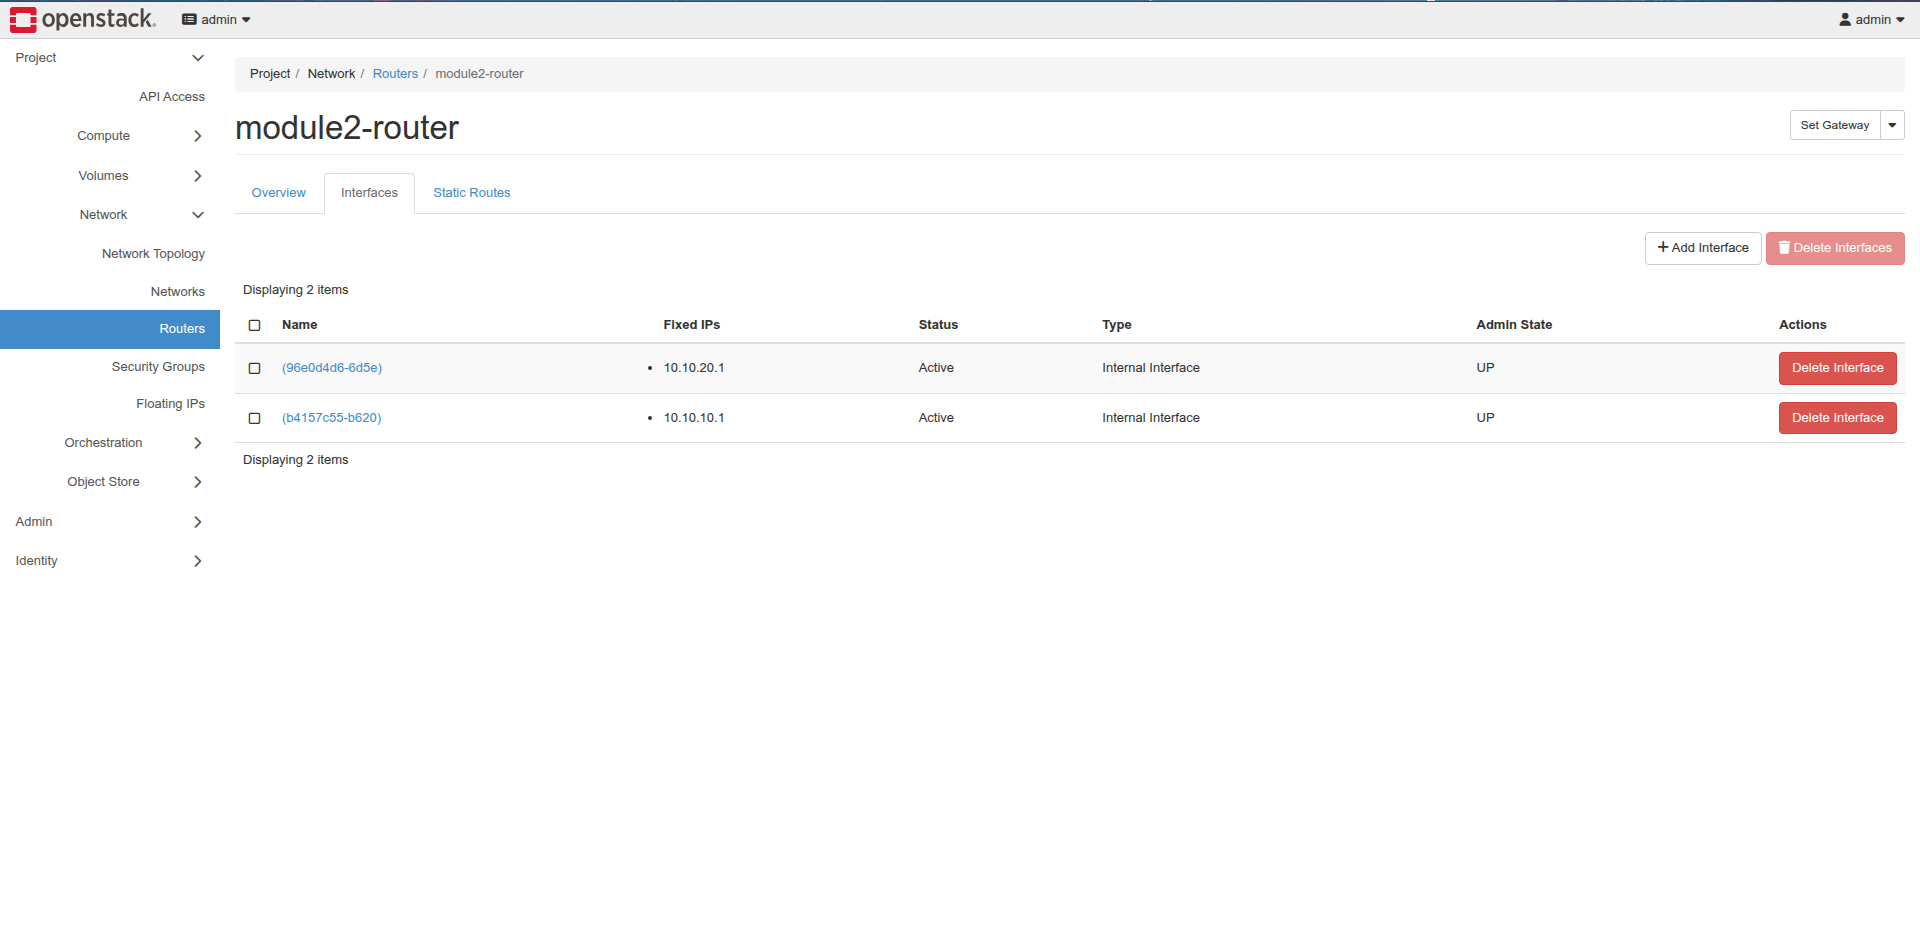
\includegraphics[width=0.88\linewidth]{img/m2-router-internal-interfaces.png}
\caption{Hai cổng giao diện nội bộ (\texttt{10.10.10.1} và \texttt{10.10.20.1}) gắn vào \texttt{module2-router}.}
\label{fig:m2_router_interfaces}
\end{figure}

\begin{itemize}
    \item \textbf{Bảng Phân bổ Cổng Mạng (Hình~\ref{fig:m2_ports}):} Danh sách cổng ảo trong Neutron phản ánh đầy đủ các thành phần hạ tầng, bao gồm cổng dành cho DHCP Agent phục vụ cấp phát IP tự động và các cổng Gateway của router.
    \item \textbf{Sơ đồ Tô-pô Trực quan (Hình~\ref{fig:m2_topology_diagram}):} Sơ đồ tương tác trên bảng điều khiển Horizon minh họa rõ nét cấu trúc phân tầng đa lớp: luồng lưu lượng từ mạng \texttt{public} đi qua \texttt{m2-router} và rẽ nhánh an toàn vào phân vùng DMZ (đường viền đỏ) cùng phân vùng Private (đường viền xanh lá).
\end{itemize}

\begin{figure}[H]
\centering
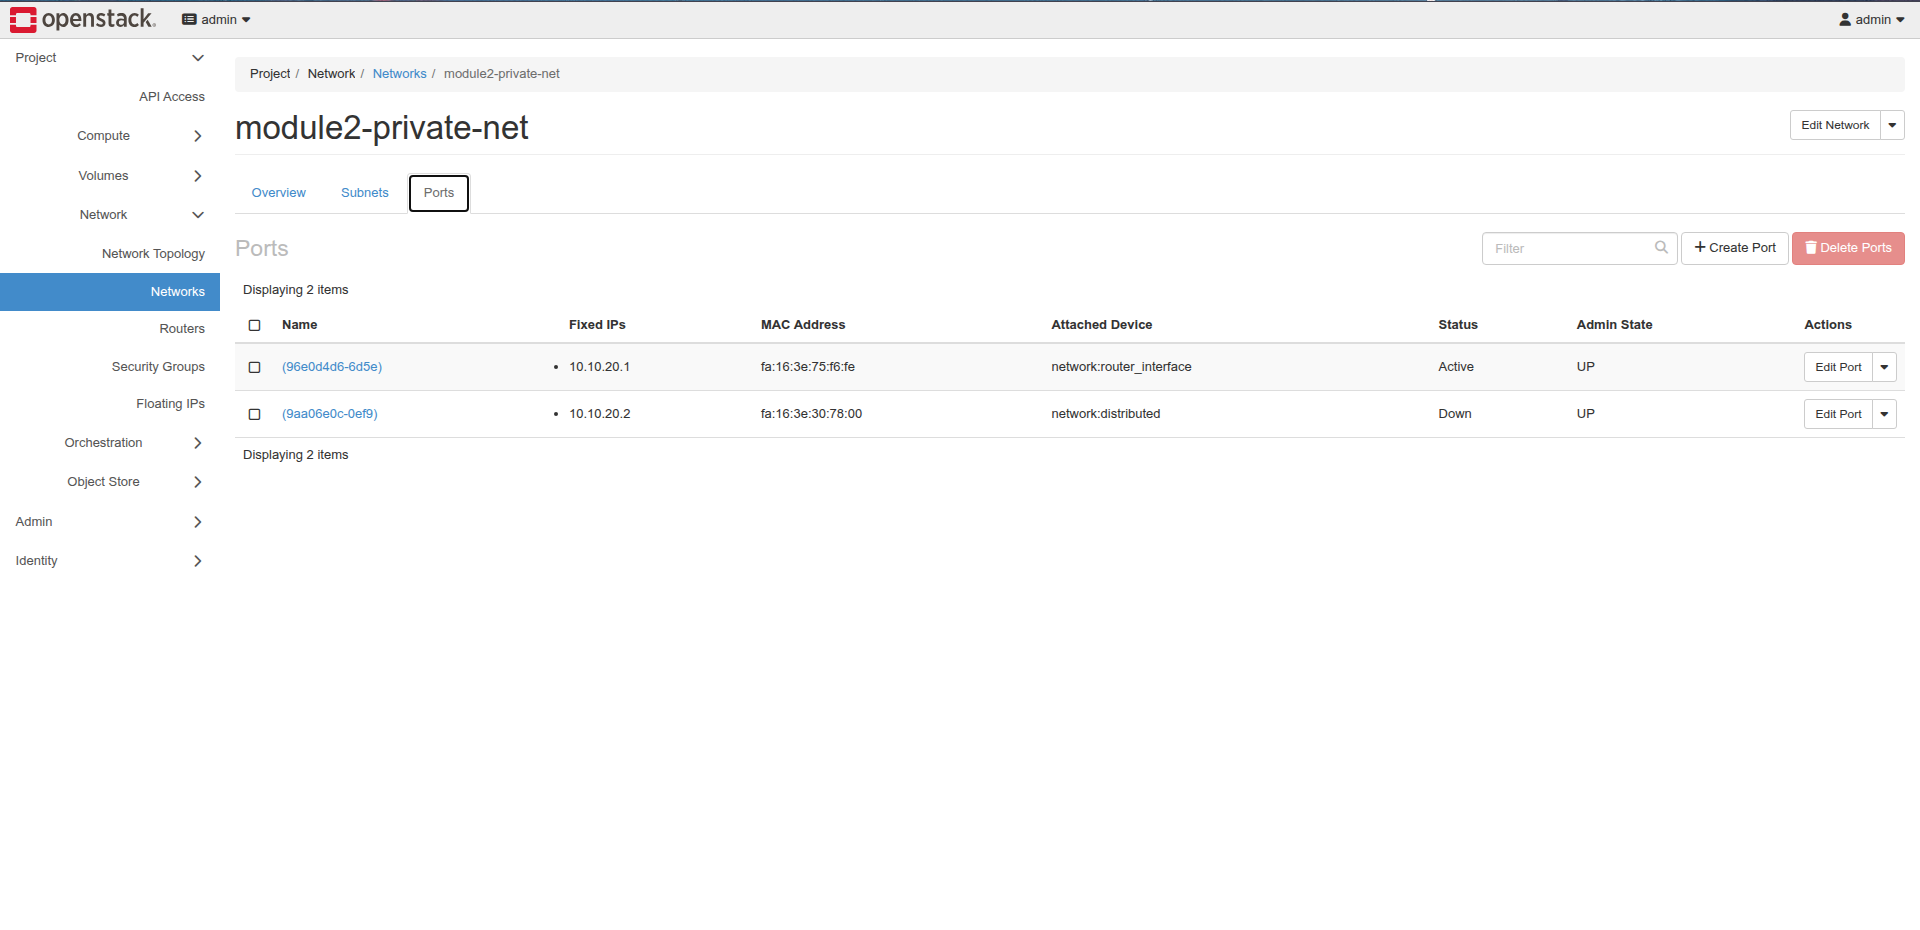
\includegraphics[width=0.88\linewidth]{img/m2-ports-list.png}
\caption{Danh sách cổng mạng trên \texttt{m2-private-net} gồm router gateway và DHCP agent.}
\label{fig:m2_ports}
\end{figure}

\begin{figure}[H]
\centering
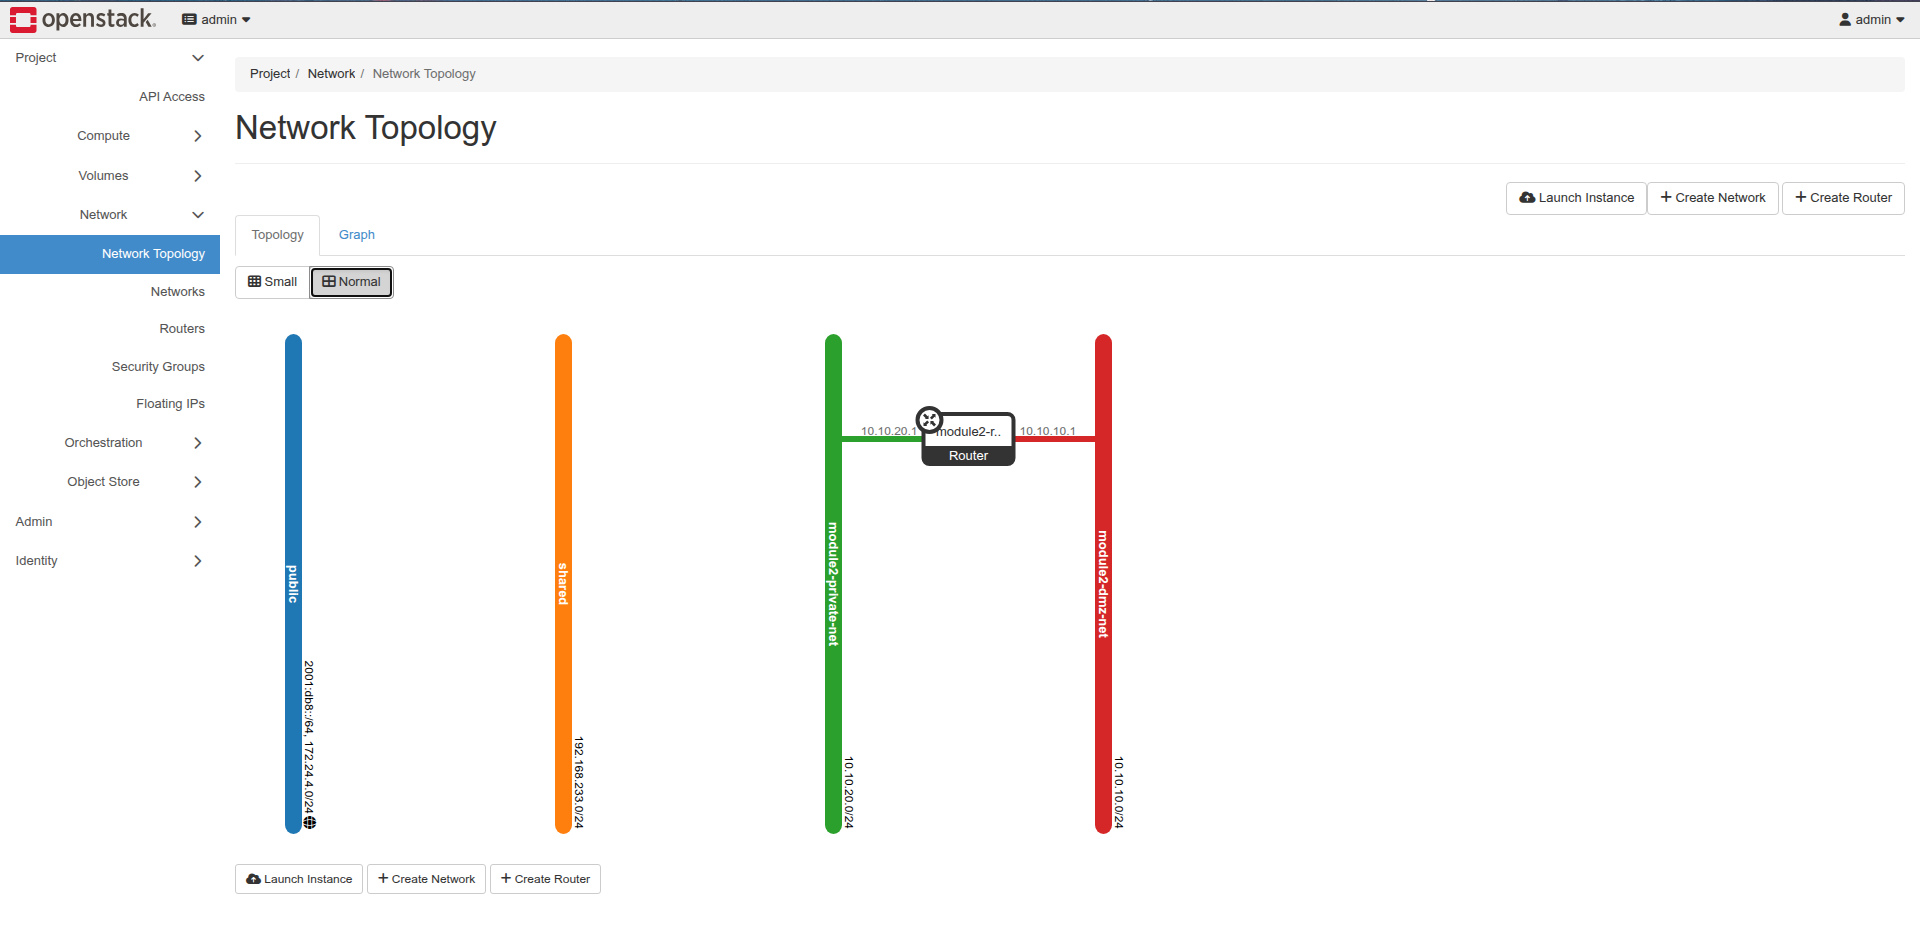
\includegraphics[width=0.88\linewidth]{img/m2-network-topology-diagram.png}
\caption{Sơ đồ tô-pô mạng trực quan trên Horizon thể hiện kiến trúc định tuyến L3.}
\label{fig:m2_topology_diagram}
\end{figure}

\newpage

\section{Module 3: Máy ảo Đa Card mạng \& Xử lý Định tuyến Bất đối xứng}

\subsection{Mục tiêu \& Thách thức Kiến trúc Định tuyến}
Trong Module 3, nhóm chúng em triển khai một máy ảo đóng vai trò Application Gateway gắn đồng thời vào cả hai phân đoạn mạng DMZ và Private. Trong quá trình thực nghiệm các hệ thống đa card mạng (Multi-Homed), một thách thức kỹ thuật lớn mà nhóm gặp phải chính là hiện tượng \textbf{định tuyến bất đối xứng} (Asymmetric Routing, mô tả tại Hình~\ref{fig:m3_asymm_concept}): gói tin yêu cầu chiều vào (Ingress) được gửi tới Floating IP và đi qua cổng DMZ, nhưng gói tin phản hồi chiều ra (Egress) lại bị hệ điều hành gửi nhầm qua cổng Private theo bảng định tuyến mặc định. Kết quả là tường lửa kiểm tra trạng thái (Stateful Firewall/Conntrack) trên Neutron Router coi đây là luồng gói tin không hợp lệ và lập tức hủy bỏ (drop) kết nối.

\begin{figure}[H]
\centering
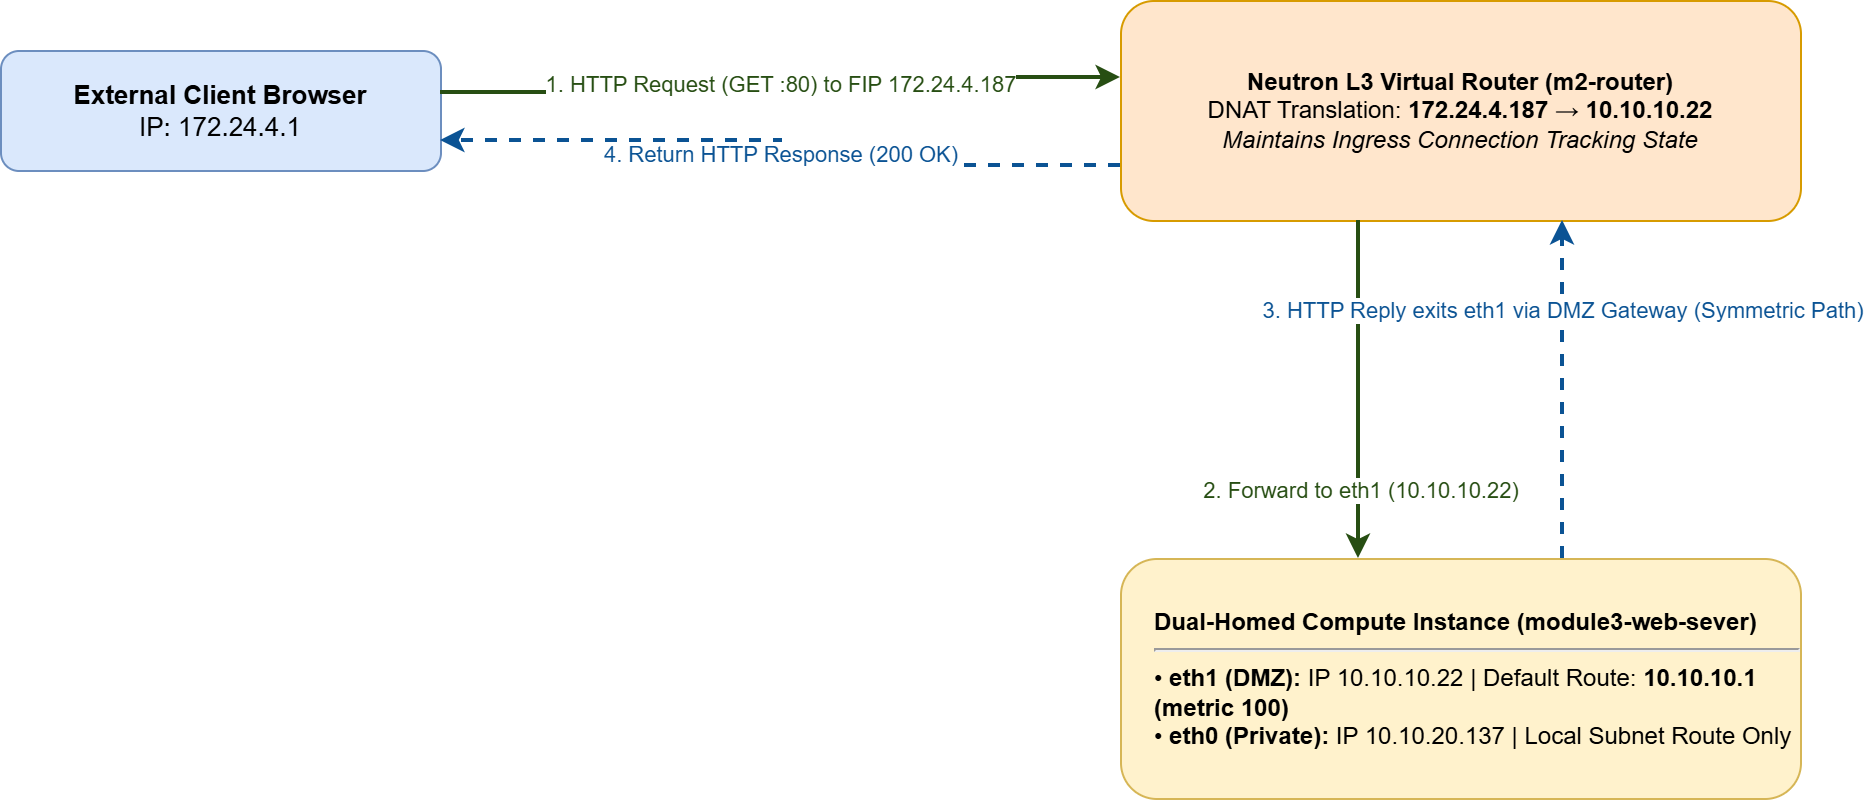
\includegraphics[width=0.92\linewidth]{img/routing_traffic_flow.png}
\caption{Luồng gói tin Ingress và Egress của máy ảo web đa card mạng dưới sự kiểm soát định tuyến đối xứng.}
\label{fig:m3_asymm_concept}
\end{figure}

\subsection{Quy trình Triển khai}
Nhóm chúng em thực hiện quy trình triển khai theo các bước sau:
\begin{enumerate}
    \item \textbf{Khởi tạo Nhóm Bảo mật (\texttt{module3-web-sg}):}
    Nhóm thiết lập Security Group chuyên biệt với các luật cho phép lưu lượng SSH (TCP cổng 22), HTTP (TCP cổng 80) và giao thức ICMP (Ping) từ mọi dải địa chỉ IPv4 (\nolinkurl{0.0.0.0/0}), như minh họa tại Hình~\ref{fig:m3_secgroup_rules}.
    
    \item \textbf{Khởi tạo Máy ảo 2 Card mạng (\texttt{module3-web-sever}) (Hình~\ref{fig:m3_instance_overview}):}
    Trước khi khởi tạo máy ảo, nhóm tiến hành xác thực lại danh mục mạng tenant để đảm bảo gán đúng giao diện (Hình~\ref{fig:m3_networks_verify}). Sau đó, máy ảo được khởi chạy với 2 cổng mạng ảo chuyên dụng:
    \begin{itemize}
        \item \textbf{NIC 1 (\texttt{eth1}):} Gắn vào phân vùng \texttt{m2-dmz-net} với địa chỉ IP tĩnh \texttt{10.10.10.22}.
        \item \textbf{NIC 2 (\texttt{eth0}):} Gắn vào phân vùng \texttt{m2-private-net} với địa chỉ IP tĩnh \texttt{10.10.20.137}.
    \end{itemize}

    \item \textbf{Gán Địa chỉ IP Nổi (Floating IP):}
    Nhóm xin cấp phát địa chỉ IP công khai \texttt{172.24.4.187} từ pool mạng \texttt{public} và thực hiện ánh xạ \textbf{chính xác vào cổng DMZ} (\texttt{10.10.10.22}) thay vì cổng Private (Hình~\ref{fig:m3_floating_ip}).
\end{enumerate}

\begin{figure}[H]
\centering
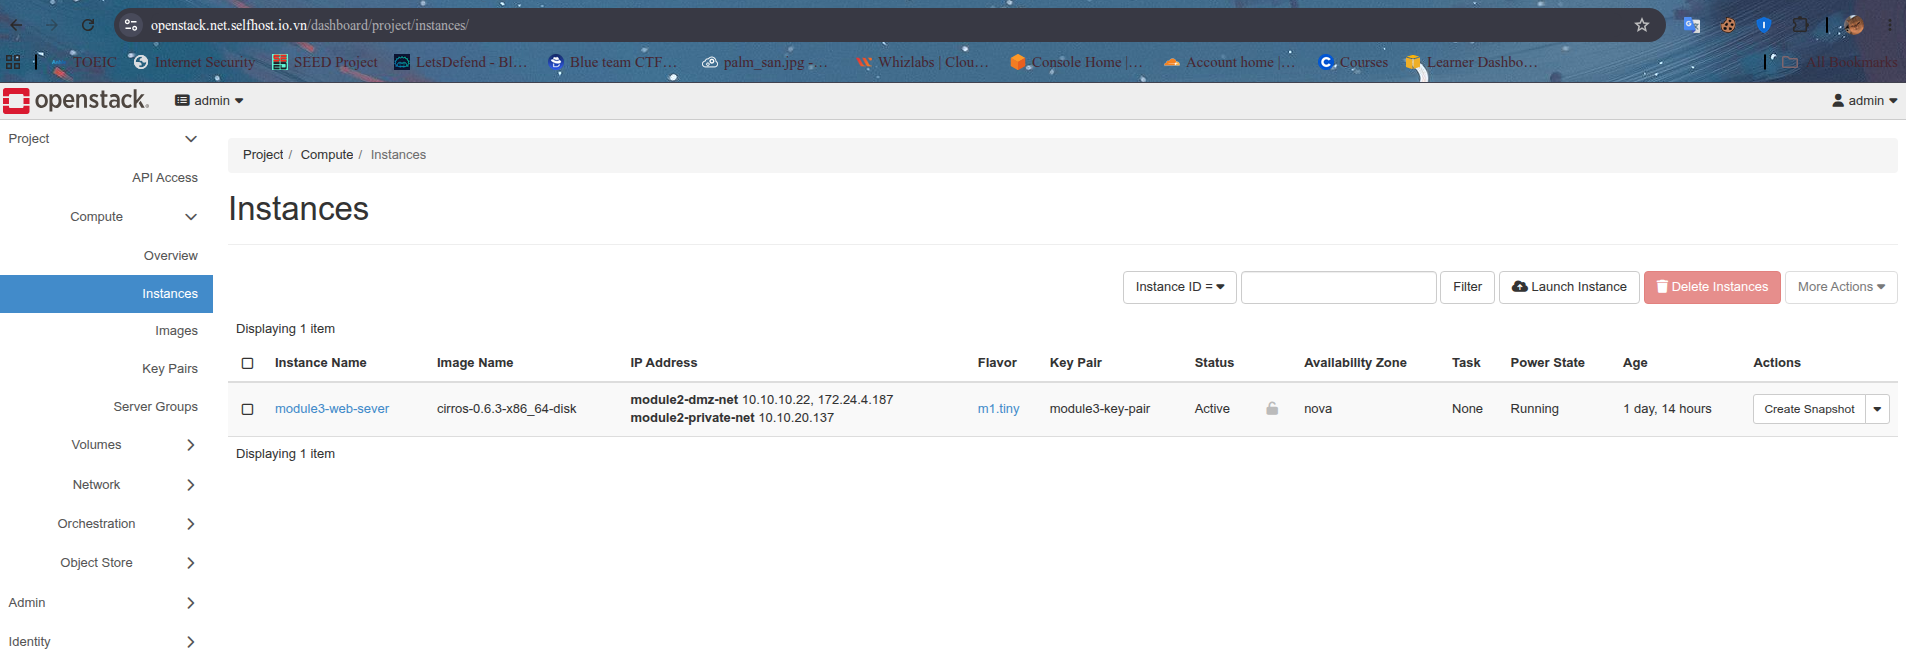
\includegraphics[width=0.88\linewidth]{img/m3-instance-dual-homed-overview.png}
\caption{Máy ảo \texttt{module3-web-sever} gắn đồng thời 2 card mạng DMZ và Private.}
\label{fig:m3_instance_overview}
\end{figure}

\begin{figure}[H]
\centering
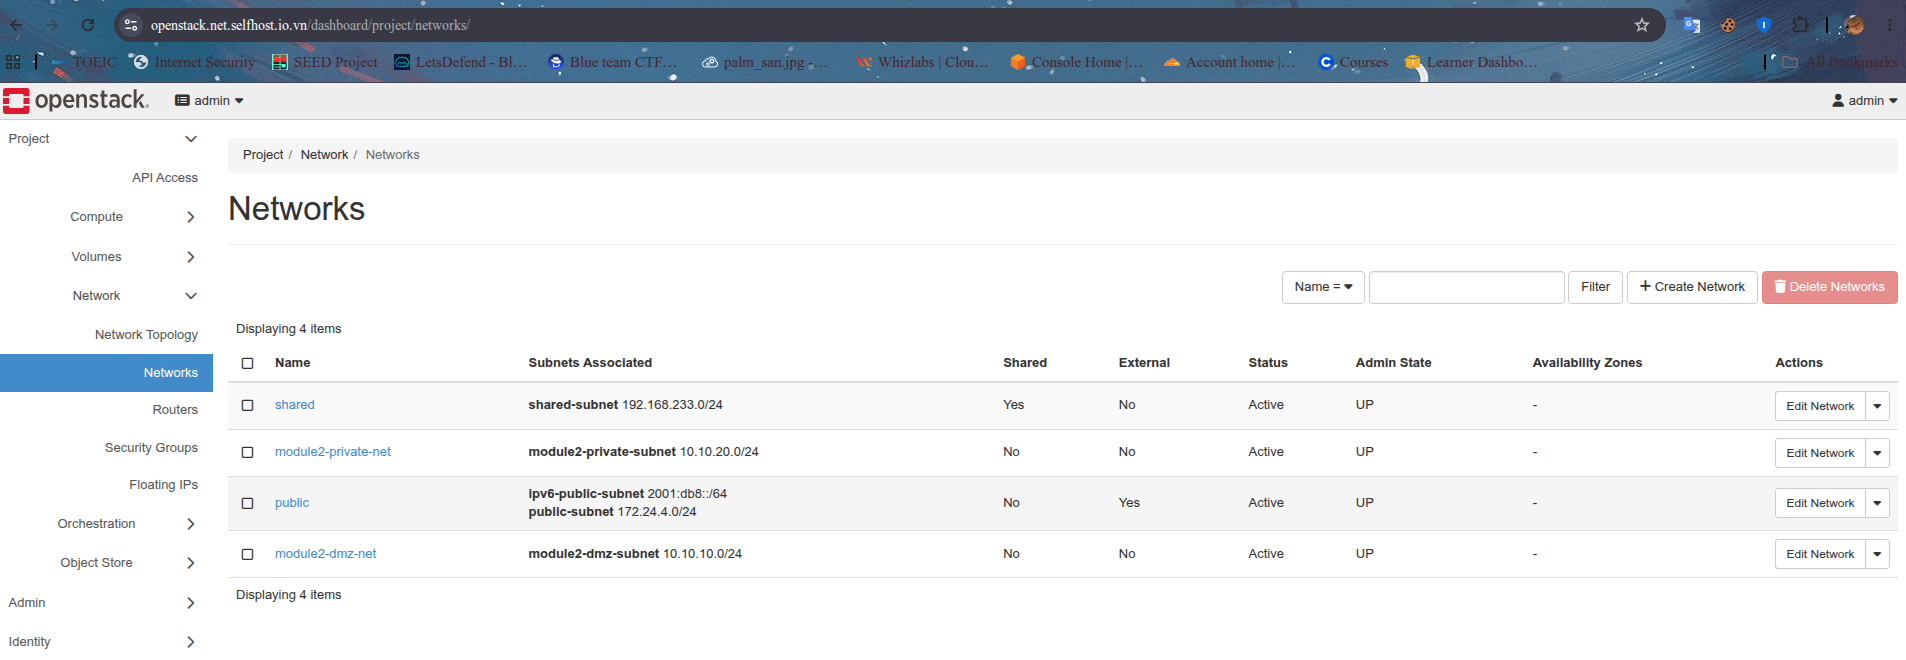
\includegraphics[width=0.88\linewidth]{img/m3-network-inventory.png}
\caption{Xác nhận bảng danh mục mạng tenant trước khi đính kèm máy ảo.}
\label{fig:m3_networks_verify}
\end{figure}

\begin{figure}[H]
\centering
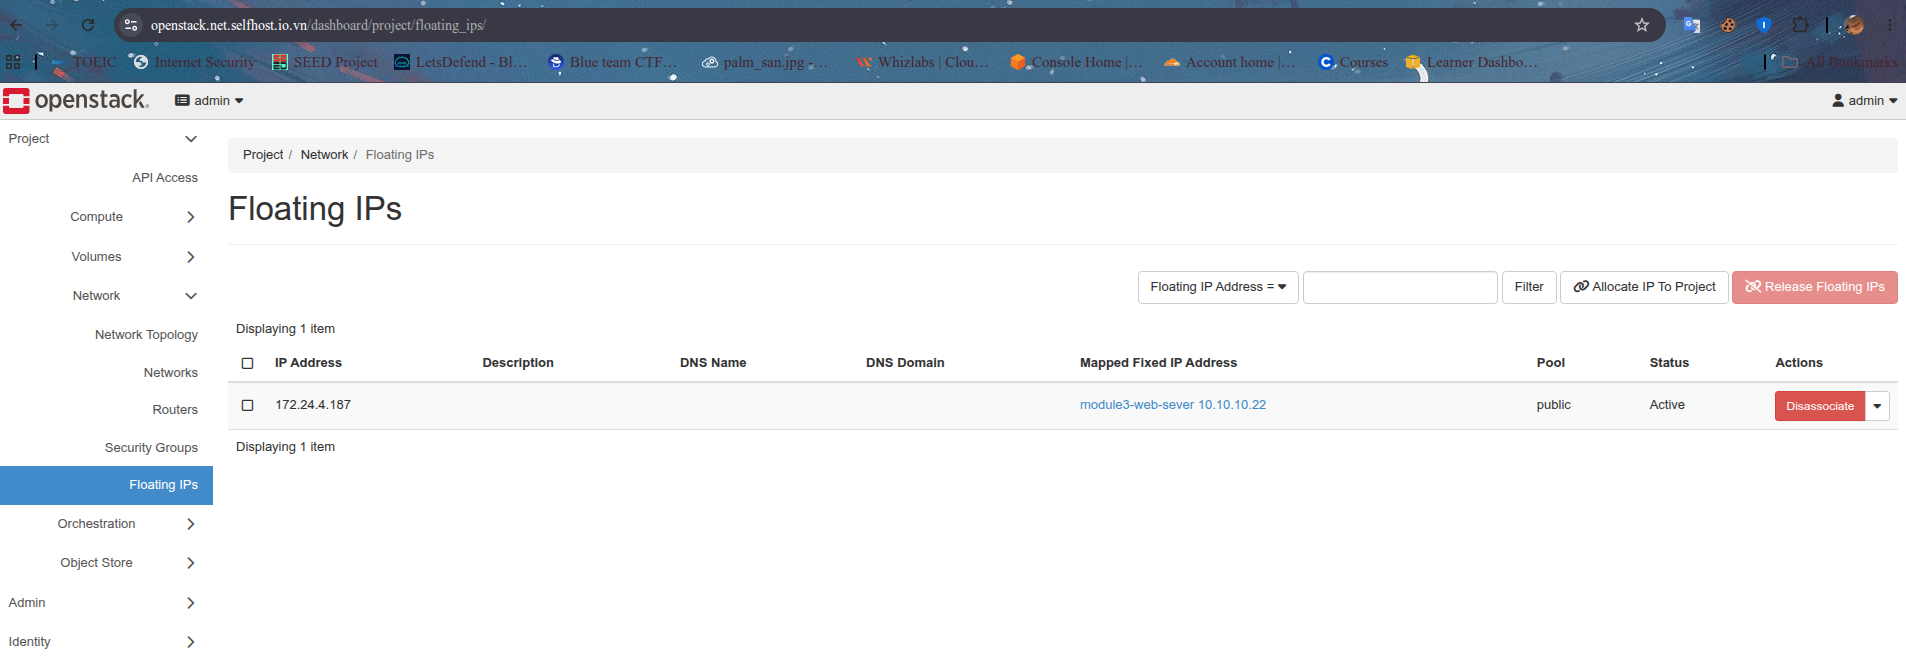
\includegraphics[width=0.88\linewidth]{img/m3-floating-ip-mapping.png}
\caption{Floating IP \texttt{172.24.4.187} ánh xạ chính xác vào IP cố định DMZ \texttt{10.10.10.22}.}
\label{fig:m3_floating_ip}
\end{figure}

\begin{figure}[H]
\centering
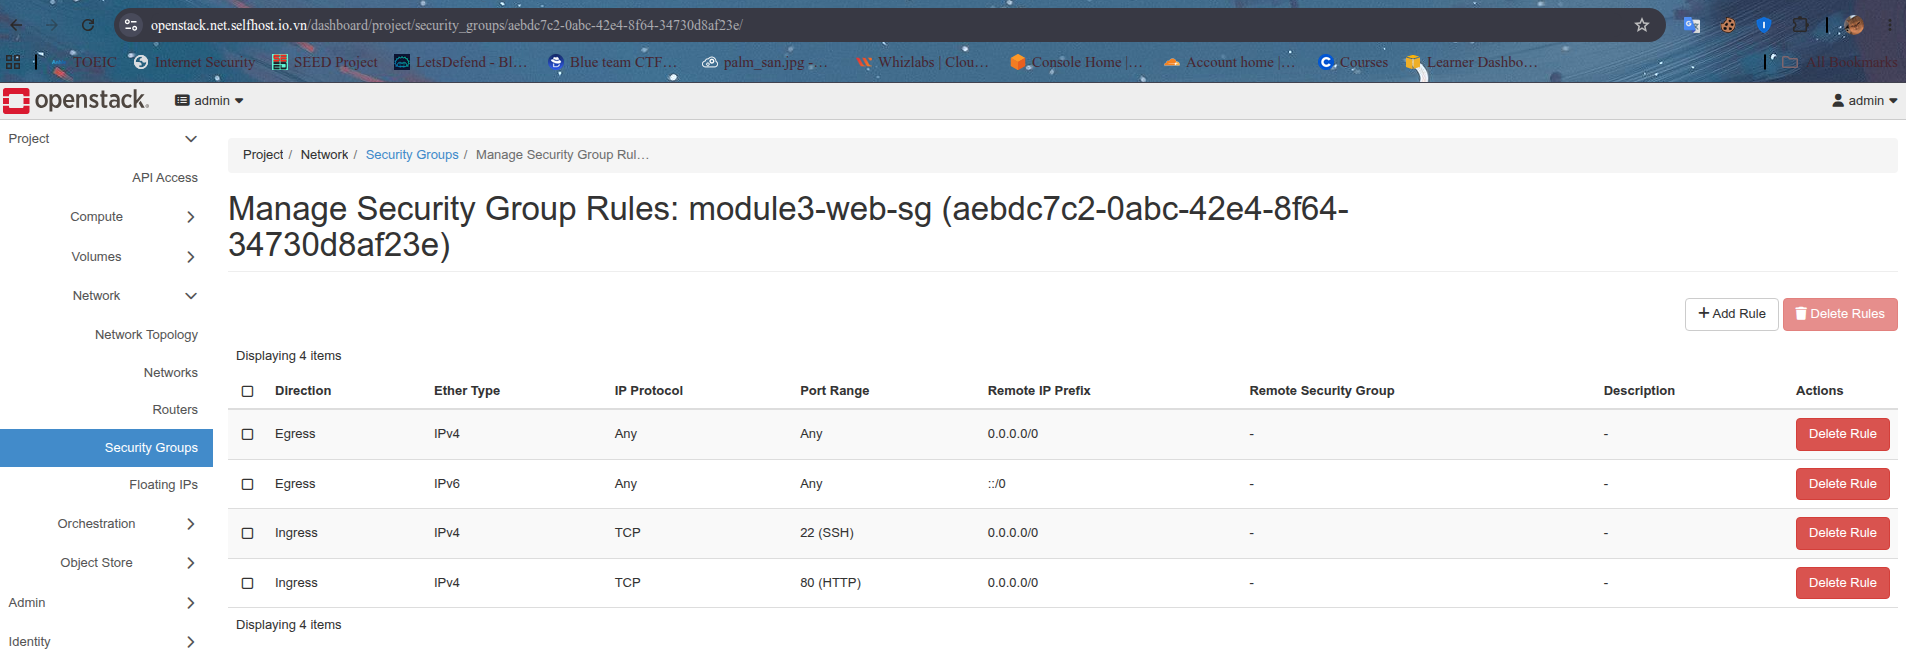
\includegraphics[width=0.88\linewidth]{img/m3-security-group-rules.png}
\caption{Luật tường lửa Security Group \texttt{module3-web-sg} mở các cổng 22, 80 và ICMP.}
\label{fig:m3_secgroup_rules}
\end{figure}

\subsection{Cấu hình Bảng Định tuyến Kernel \& Kiểm thử Dịch vụ Web}
Sau khi truy cập vào console của máy ảo qua SSH, nhóm chúng em kiểm tra thông số mạng và phát hiện vấn đề định tuyến thực tế (Hình~\ref{fig:m3_ip_route}):
\begin{itemize}
    \item Qua lệnh \texttt{ip addr}, nhóm xác nhận cổng \texttt{eth0} nhận địa chỉ \nolinkurl{10.10.20.137/24} (Private) và cổng \texttt{eth1} nhận địa chỉ \nolinkurl{10.10.10.22/24} (DMZ).
    \item Tuy nhiên, DHCP mặc định đã thiết lập Default Gateway trỏ qua giao diện \texttt{eth0} (mạng Private). Để xử lý triệt để hiện tượng định tuyến bất đối xứng và tránh bị Router hủy gói tin do lệch phiên theo dõi conntrack, nhóm chúng em đã cấu hình lại bảng định tuyến của nhân Linux nhằm ưu tiên Default Gateway đi qua cổng DMZ:
\begin{lstlisting}[language=bash]
$ sudo ip route replace default via 10.10.10.1 dev eth1 metric 100
\end{lstlisting}
    Quy tắc này bảo đảm mọi gói tin phản hồi ra bên ngoài (đặc biệt là lưu lượng HTTP) đều bắt buộc đi ngược lại qua cổng DMZ (\texttt{eth1}), nơi bảng phiên dịch địa chỉ (DNAT/SNAT) của Neutron Router đang duy trì trạng thái phiên.
\end{itemize}

\begin{figure}[H]
\centering
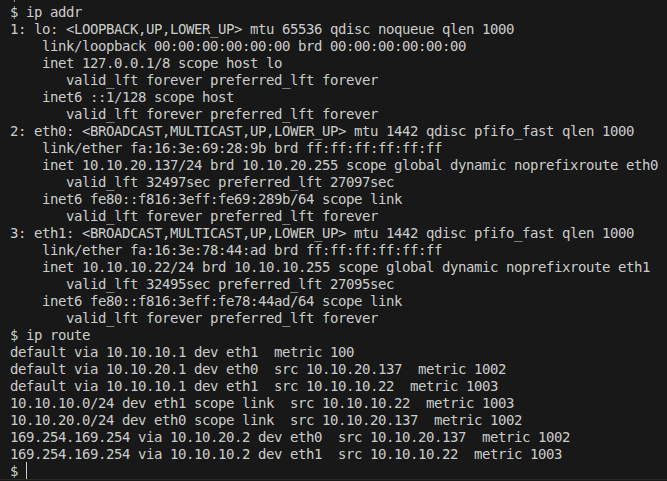
\includegraphics[width=0.88\linewidth]{img/m3-instance-ip-route-terminal.png}
\caption{Cấu hình mạng nội bộ máy ảo (\texttt{ip addr}) và bảng định tuyến kernel (\texttt{ip route}).}
\label{fig:m3_ip_route}
\end{figure}

\noindent \textbf{Khởi chạy Dịch vụ \& Nghiệm thu Toàn trình:}
Để kiểm thử khả năng cung cấp dịch vụ web ra ngoài Internet, nhóm chúng em khởi chạy web server bằng lệnh \texttt{sudo busybox httpd -f -p 80 -v}. Từ máy client bên ngoài, nhóm tiến hành gửi yêu cầu HTTP đến địa chỉ Floating IP \url{http://172.24.4.187}. Kết quả thực nghiệm ghi nhận nhật ký truy cập (access log) hiển thị đầy đủ trên terminal của máy chủ (Hình~\ref{fig:m3_busybox_logs}), đồng thời giao diện web được tải và render thành công trên trình duyệt của máy khách (Hình~\ref{fig:m3_browser_http}), chứng minh giải pháp xử lý định tuyến đối xứng hoạt động hoàn toàn chính xác.

\begin{figure}[H]
\centering
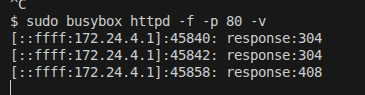
\includegraphics[width=0.88\linewidth]{img/m3-busybox-httpd-logs.png}
\caption{Nhật ký truy cập của tiến trình BusyBox HTTP daemon ghi nhận yêu cầu từ client.}
\label{fig:m3_busybox_logs}
\end{figure}

\begin{figure}[H]
\centering
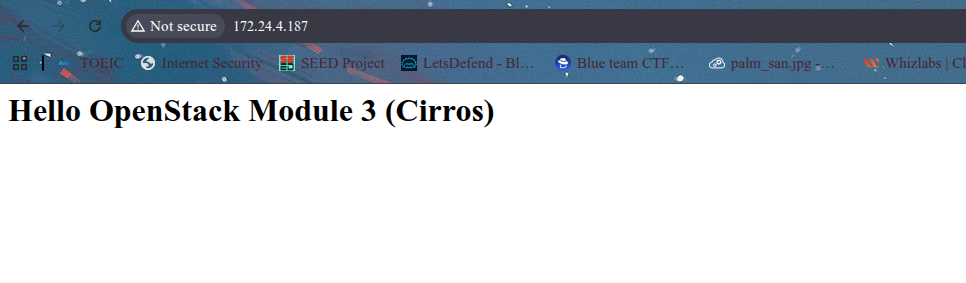
\includegraphics[width=0.88\linewidth]{img/m3-web-browser-http-verification.png}
\caption{Kiểm thử truy cập dịch vụ web thành công qua trình duyệt với Floating IP \texttt{172.24.4.187}.}
\label{fig:m3_browser_http}
\end{figure}

\newpage

\section{Module 4: Lưu trữ Bền vững \& Phục hồi Thảm họa với Snapshot}

\subsection{Mục tiêu \& Mô hình Lưu trữ Lai (Hybrid Storage)}
Trong kiến trúc điện toán đám mây hiện đại, nguyên lý cốt lõi là tách biệt hoàn toàn giữa các nút tính toán tạm thời (Ephemeral Compute Nodes) và lớp lưu trữ trạng thái bền vững (Persistent Storage State). Để hiện thực hóa mô hình này, nhóm chúng em triển khai kiến trúc lưu trữ lai (Hybrid Storage Model) kết hợp linh hoạt giữa hai dịch vụ nền tảng của OpenStack:
\begin{itemize}
    \item \textbf{Lưu trữ Đối tượng (OpenStack Swift)~\cite{swift_storage}:} Đóng vai trò kho lưu trữ tài nguyên phi cấu trúc và các gói phân phối mã nguồn tĩnh thông qua giao thức RESTful API, cho phép các tiến trình máy ảo truy xuất nhanh qua HTTP.
    \item \textbf{Lưu trữ Khối (OpenStack Cinder)~\cite{cinder_storage}:} Cung cấp các thiết bị khối chuẩn POSIX với độ trễ thấp và băng thông cao, được gắn trực tiếp vào máy ảo làm không gian thực thi dữ liệu ứng dụng.
    \item \textbf{Cơ chế Phục hồi Thảm họa (Snapshot Lifecycle):} Thực hiện chụp ảnh trạng thái ổ đĩa theo thời điểm (Point-in-time Snapshot), làm tiền đề cho việc nhân bản môi trường hoặc khôi phục dữ liệu tức thời khi máy ảo tính toán gặp sự cố phần cứng.
\end{itemize}

\subsection{Thiết lập Swift Object Storage}
Bước đầu tiên trong quy trình, nhóm chúng em tiến hành thiết lập OpenStack Swift để làm kênh phân phối mã nguồn cho ứng dụng:
\begin{itemize}
    \item \textbf{Khởi tạo Container:} Chúng em tạo một container chuyên dụng mang tên \nolinkurl{module4-tetris-src} áp dụng chính sách lưu trữ mặc định \texttt{Policy-0}, đồng thời thiết lập quyền truy cập đọc công khai (\nolinkurl{Read-ACL=.r:*}) nhằm cho phép các node trong mạng nội bộ tải tài nguyên mà không cần truyền token xác thực phức tạp.
    \item \textbf{Tải lên Đối tượng:} Tệp mã nguồn giao diện \texttt{index.html} (kích thước 247 bytes) được nhóm chúng em tải trực tiếp lên container và kiểm tra tính sẵn sàng thông qua giao diện dòng lệnh (Hình~\ref{fig:m4_swift_upload}).
\end{itemize}

\begin{figure}[H]
\centering
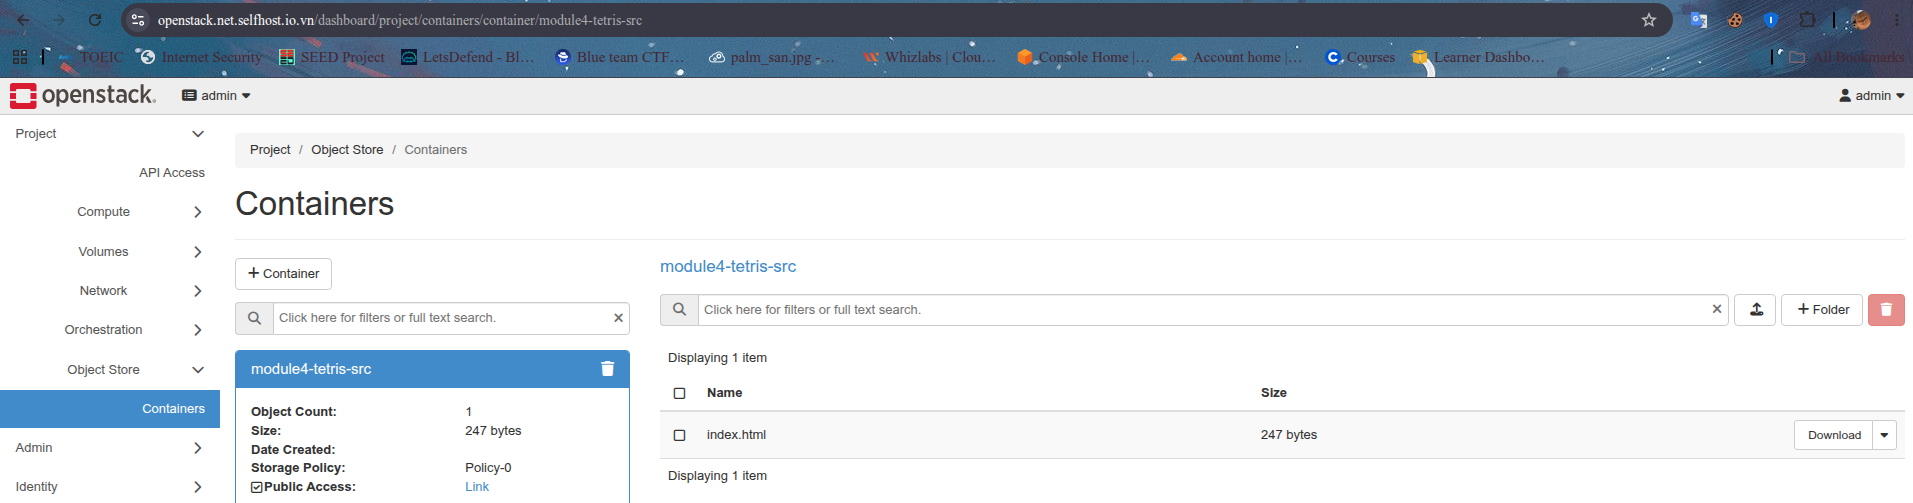
\includegraphics[width=0.88\linewidth]{img/m4-swift-container-object-upload.png}
\caption{Container Swift \texttt{module4-tetris-src} lưu trữ tệp \texttt{index.html} với quyền truy cập public.}
\label{fig:m4_swift_upload}
\end{figure}

\subsection{Tích hợp Cinder Block Volume \& Triển khai Dịch vụ Web}
Sau khi hoàn tất khâu chuẩn bị mã nguồn tĩnh trên Swift, nhóm chúng em tiến hành cấp phát không gian lưu trữ khối bền vững và tích hợp vào máy chủ web:
\begin{enumerate}
    \item \textbf{Khởi tạo \& Gắn Volume:}
    Chúng em tạo một ổ đĩa Cinder dung lượng 1 GiB với định danh \nolinkurl{module4-data-volume} và thực hiện đính kèm (attach) vào máy ảo \texttt{module3-web-sever}. Lớp ảo hóa KVM/QEMU nhận diện thiết bị này dưới định danh \texttt{/dev/vdc} (Hình~\ref{fig:m4_cinder_volume}).
    
    \item \textbf{Định dạng Hệ thống Tệp \& Đồng bộ Mã nguồn (Hình~\ref{fig:m4_vm1_workflow}):}
    Truy cập vào máy ảo thông qua phiên SSH, nhóm chúng em tiến hành định dạng ổ đĩa với hệ thống tệp \texttt{ext4}, tạo thư mục mount \texttt{/mnt/data}, sau đó tải tệp mã nguồn từ endpoint REST của Swift về lưu trữ trực tiếp trên volume:
\begin{lstlisting}[language=bash, basicstyle=\ttfamily\scriptsize]
$ sudo mkfs.ext4 /dev/vdc
$ sudo mkdir -p /mnt/data && sudo mount /dev/vdc /mnt/data
$ cd /mnt/data
$ sudo wget http://192.168.2.10:8080/v1/AUTH_.../module4-tetris-src/index.html
\end{lstlisting}

    \item \textbf{Kích hoạt \& Kiểm thử Dịch vụ Web:}
    Để ứng dụng phục vụ trực tiếp từ ổ đĩa bền vững, chúng em khởi chạy tiến trình BusyBox HTTP daemon với thư mục gốc trỏ vào \texttt{/mnt/data}:
\begin{lstlisting}[language=bash, basicstyle=\ttfamily\scriptsize]
$ sudo busybox httpd -f -p 80 -h /mnt/data &
$ curl http://127.0.0.1
\end{lstlisting}
    Kết quả kiểm tra qua lệnh \texttt{curl} xác nhận máy chủ web đã phản hồi chính xác nội dung HTML được đọc từ phân vùng Cinder.
\end{enumerate}

\begin{figure}[H]
\centering
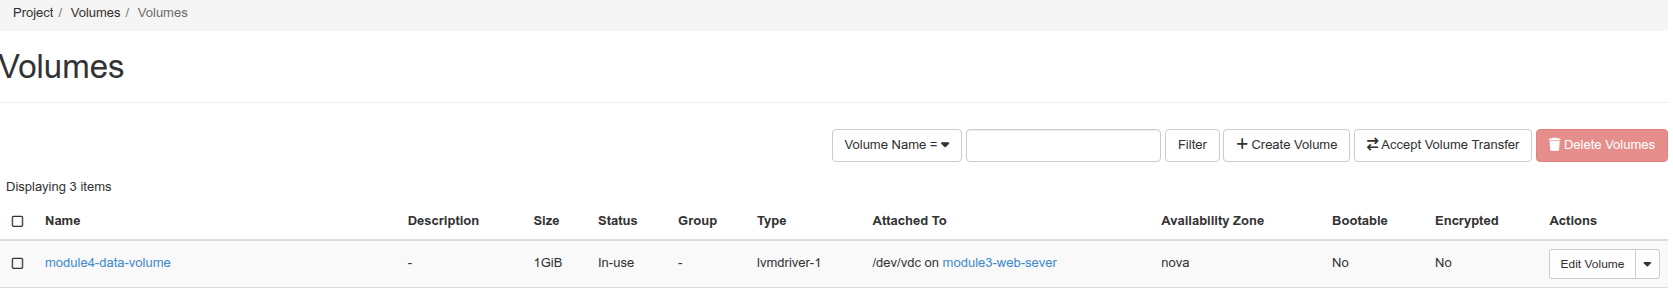
\includegraphics[width=0.88\linewidth]{img/m4-cinder-volume-attached.png}
\caption{Cinder volume \nolinkurl{module4-data-volume} (1 GiB) ở trạng thái In-Use gắn vào \nolinkurl{module3-web-sever}.}
\label{fig:m4_cinder_volume}
\end{figure}

\begin{figure}[H]
\centering
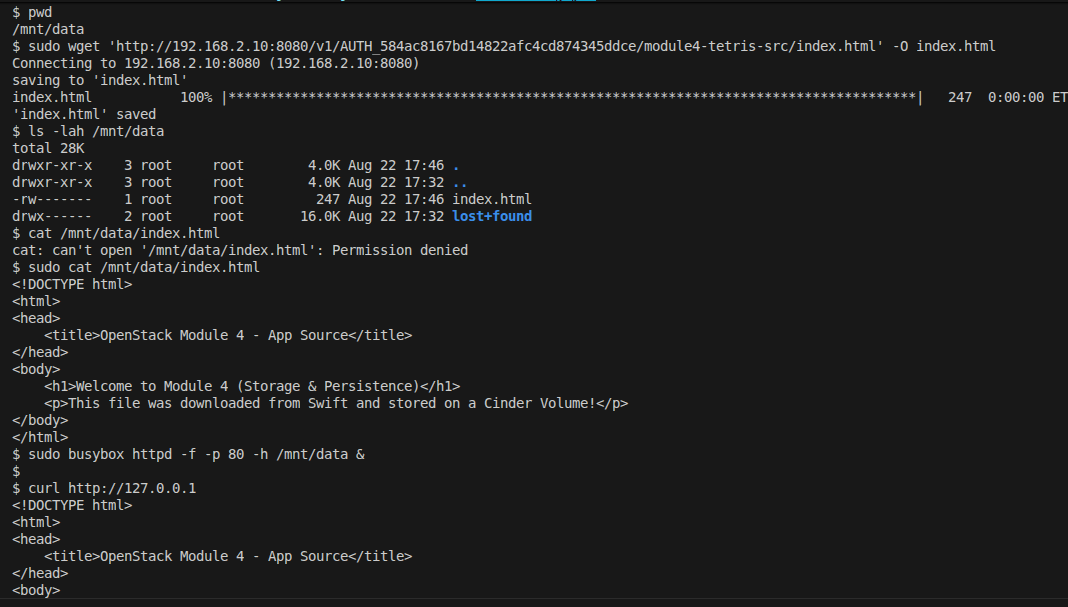
\includegraphics[width=0.88\linewidth]{img/m4-vm1-swift-fetch-cinder-host.png}
\caption{Quy trình terminal: tải mã nguồn từ Swift, mount ổ đĩa Cinder và chạy dịch vụ web.}
\label{fig:m4_vm1_workflow}
\end{figure}

\subsection{Tạo Snapshot \& Xác thực Phục hồi Thảm họa (Disaster Recovery)}
Nhằm chứng minh khả năng bảo toàn dữ liệu và phục hồi hệ thống khi xảy ra sự cố nghiêm trọng trên máy chủ tính toán, nhóm chúng em xây dựng kịch bản cứu hộ dữ liệu độc lập thông qua Snapshot:
\begin{enumerate}
    \item \textbf{Ngắt Kết nối An toàn \& Tạo Snapshot:}
    Để đảm bảo tính toàn vẹn dữ liệu (Data Consistency), chúng em tiến hành unmount hệ thống tệp và detach ổ đĩa khỏi máy ảo ban đầu. Tiếp theo, một bản sao lưu trạng thái thời điểm mang tên \texttt{module4-data-snapshot} (1 GiB) được khởi tạo thành công (Hình~\ref{fig:m4_volume_snapshot}).
    
    \item \textbf{Khôi phục Volume Độc lập từ Snapshot:}
    Từ bản snapshot vừa ghi lại, chúng em tạo ra một ổ đĩa khối mới hoàn toàn độc lập mang tên \nolinkurl{module4-restored-volume}.

    \item \textbf{Khởi tạo Máy ảo Phục hồi Cứu hộ:}
    Chúng em triển khai một máy ảo cứu hộ mới mang tên \nolinkurl{module4-recovery-server} (sử dụng image Fedora Cloud Base) trên phân đoạn mạng \texttt{m2-dmz-net}, sau đó gắn ổ đĩa \nolinkurl{module4-restored-volume} vào máy ảo này.

    \item \textbf{Kiểm tra Tính Toàn vẹn Dữ liệu Cấp độ Byte (Hình~\ref{fig:m4_recovery_verify}):}
    Trên máy ảo phục hồi, nhóm chúng em mount trực tiếp thiết bị \texttt{/dev/vdb} vào thư mục \texttt{/mnt/recovered} mà \textbf{hoàn toàn không cần format lại hệ thống tệp}:
\begin{lstlisting}[language=bash, basicstyle=\ttfamily\scriptsize]
[fedora@module4-recovery-server ~]$ sudo mount /dev/vdb /mnt/recovered
[fedora@module4-recovery-server ~]$ sudo cat /mnt/recovered/index.html
\end{lstlisting}
    Nội dung tệp \texttt{index.html} được đọc ra chính xác tuyệt đối từng byte. Thực nghiệm này chứng minh cơ chế Snapshot của Cinder bảo vệ dữ liệu nguyên vẹn 100\%, giúp hệ thống sẵn sàng phục hồi ngay cả khi node tính toán ban đầu bị phá hủy hoàn toàn.
\end{enumerate}

\begin{figure}[H]
\centering
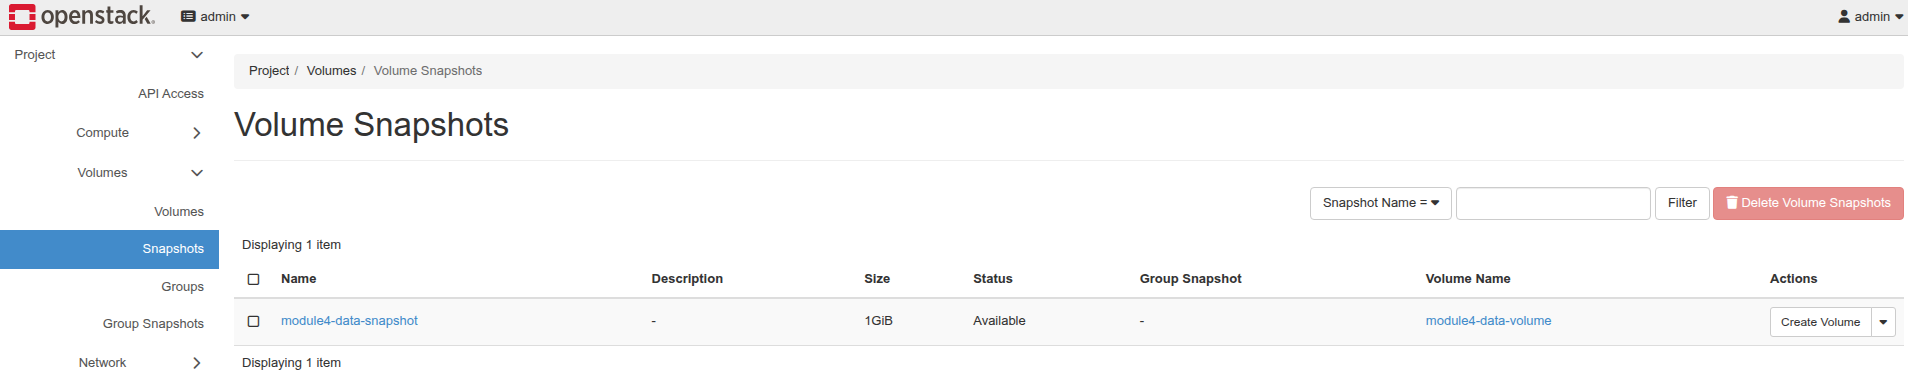
\includegraphics[width=0.88\linewidth]{img/m4-cinder-volume-snapshot.png}
\caption{Bản snapshot \texttt{module4-data-snapshot} ghi nhận trạng thái ổ đĩa tại thời điểm sao lưu.}
\label{fig:m4_volume_snapshot}
\end{figure}

\begin{figure}[H]
\centering
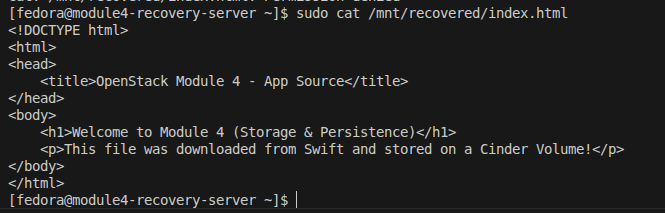
\includegraphics[width=0.88\linewidth]{img/m4-recovery-server-data-verification.png}
\caption{Kiểm tra tính toàn vẹn trên máy ảo phục hồi xác nhận dữ liệu được bảo toàn nguyên vẹn.}
\label{fig:m4_recovery_verify}
\end{figure}



\newpage

\section{Module 5: Tự động hóa Khai báo Hạ tầng với OpenStack Heat}

\subsection{Mục tiêu \& Mô hình Hạ tầng dưới dạng Mã (IaC)}
Nếu như ở các Module từ 1 đến 4, nhóm chúng em đã tìm hiểu và làm quen với quy trình quản trị hạ tầng theo từng bước mệnh lệnh thủ công (Imperative Approach), thì trong môi trường doanh nghiệp quy mô lớn, phương pháp này bộc lộ nhiều hạn chế về thời gian triển khai, khó kiểm soát phiên bản và dễ phát sinh sai sót do con người. Để khắc phục triệt để, tại Module 5, nhóm chúng em áp dụng mô hình Hạ tầng dưới dạng Mã (Infrastructure as Code - IaC) thông qua công cụ điều phối \textbf{OpenStack Heat Orchestration Engine}~\cite{heat_hot_guide}.

Bằng phương pháp tiếp cận khai báo (Declarative Approach), toàn bộ kiến trúc hạ tầng phức tạp bao gồm: mạng ảo Neutron, router L3, security group, cổng mạng, địa chỉ Floating IP, ổ đĩa Cinder, máy ảo Nova và kịch bản nạp ứng dụng tự động qua Cloud-Init~\cite{cloudinit_docs} đều được chúng em gói gọn bên trong một tệp mẫu duy nhất mang tên \texttt{module5\_service.yaml}.

\subsection{Cấu trúc Mẫu Điều phối Heat (HOT Architecture)}
Mẫu template được nhóm chúng em xây dựng tuân thủ quy chuẩn phiên bản \nolinkurl{heat_template_version: 2021-04-16}. Khi tiếp nhận bản khai báo này, Heat Engine sẽ tự động phân tích các hàm liên kết nội tại (như \texttt{get\_resource} và \texttt{get\_param}) để xây dựng một Đồ thị có hướng không chu trình (Directed Acyclic Graph - DAG), từ đó tối ưu hóa thứ tự cấp phát song song cho 10 khối tài nguyên liên kết chặt chẽ:

\begin{lstlisting}[language=yaml, basicstyle=\ttfamily\scriptsize, caption={Khai báo tài nguyên trong Heat Template (\texttt{module5\_service.yaml}).}]
heat_template_version: 2021-04-16
description: Complete automated stack with network, storage, VM, and cloud-init.

parameters:
  image: { type: string, default: Fedora-Cloud-Base-37-1.7.x86_64 }
  flavor: { type: string, default: m1.small }
  key_name: { type: string, default: module3-key-pair }
  public_network: { type: string, default: public }

resources:
  m5_dmz_net:
    type: OS::Neutron::Net
    properties: { name: m5-dmz-net }

  m5_dmz_subnet:
    type: OS::Neutron::Subnet
    properties:
      network: { get_resource: m5_dmz_net }
      cidr: 10.50.10.0/24
      dns_nameservers: [8.8.8.8, 1.1.1.1]

  m5_router:
    type: OS::Neutron::Router
    properties:
      external_gateway_info: { network: { get_param: public_network } }

  m5_router_interface:
    type: OS::Neutron::RouterInterface
    properties:
      router: { get_resource: m5_router }
      subnet: { get_resource: m5_dmz_subnet }

  m5_web_sg:
    type: OS::Neutron::SecurityGroup
    properties:
      rules:
        - { protocol: tcp, port_range_min: 22, port_range_max: 22 }
        - { protocol: tcp, port_range_min: 80, port_range_max: 80 }
        - { protocol: icmp }

  m5_web_port:
    type: OS::Neutron::Port
    properties:
      network: { get_resource: m5_dmz_net }
      security_groups: [{ get_resource: m5_web_sg }]

  m5_floating_ip:
    type: OS::Neutron::FloatingIP
    properties:
      floating_network: { get_param: public_network }
      port_id: { get_resource: m5_web_port }

  m5_data_volume:
    type: OS::Cinder::Volume
    properties: { name: m5-data-volume, size: 1 }

  m5_server:
    type: OS::Nova::Server
    properties:
      name: m5-web-server
      image: { get_param: image }
      flavor: { get_param: flavor }
      key_name: { get_param: key_name }
      networks: [{ port: { get_resource: m5_web_port } }]
      user_data_format: RAW
      user_data: |
        #!/bin/bash
        for i in {1..30}; do [ -b /dev/vdb ] && break; sleep 2; done
        blkid /dev/vdb || mkfs.ext4 /dev/vdb
        mkdir -p /mnt/app && mount /dev/vdb /mnt/app
        echo "<h1>Module 5 - Heat Automated Deployment</h1>" > /mnt/app/index.html
        nohup python3 -m http.server 80 --directory /mnt/app > /var/log/m5-http.log 2>&1 &

  m5_volume_attachment:
    type: OS::Cinder::VolumeAttachment
    properties:
      volume_id: { get_resource: m5_data_volume }
      instance_uuid: { get_resource: m5_server }

outputs:
  service_url:
    description: URL to access the deployed web application
    value:
      str_replace:
        template: "http://%ip%"
        params: { "%ip%": { get_attr: [m5_floating_ip, floating_ip_address] } }
\end{lstlisting}

\subsection{Pipeline Tự Cấu hình với Cloud-Init}
Một trong những giải pháp kỹ thuật trọng tâm mà nhóm chúng em thiết kế là kịch bản \texttt{user\_data} nhúng trong template, được hệ thống Cloud-Init thực thi tự động ngay khi máy ảo khởi động:
\begin{enumerate}
    \item \textbf{Vòng lặp Thăm dò Thiết bị (Storage Discovery Loop):} Do tiến trình khởi động của máy ảo diễn ra độc lập với quá trình đính kèm volume của Cinder, chúng em lập trình một vòng lặp kiểm tra trạng thái thiết bị khối \texttt{/dev/vdb} tối đa 30 lần (chu kỳ 2 giây/lần). Cơ chế này loại bỏ hoàn toàn hiện tượng tương tranh (Race Condition), đảm bảo script chỉ tiếp tục khi kernel đã nạp hoàn tất driver \texttt{virtio\_blk}.
    \item \textbf{Định dạng \& Gắn Ổ đĩa có Tính Idempotent:} Để phòng ngừa rủi ro ghi đè dữ liệu khi máy ảo tái khởi động, chúng em sử dụng lệnh \texttt{blkid /dev/vdb} kiểm tra sự tồn tại của superblock. Lệnh định dạng \texttt{mkfs.ext4} chỉ được thực thi nếu ổ đĩa hoàn toàn mới, sau đó volume được gắn an toàn vào thư mục \texttt{/mnt/app}.
    \item \textbf{Tự động Hóa Dịch vụ Web:} Kịch bản tự sinh trang giao diện HTML mẫu và kích hoạt máy chủ HTTP nền bằng Python trên cổng 80, điều hướng toàn bộ log tiến trình vào \texttt{/var/log/m5-http.log} để tiện cho việc giám sát.
\end{enumerate}

\subsection{Triển khai Stack \& Xác thực Tự động}
Trước khi khởi chạy, nhóm chúng em tiến hành kiểm tra tính hợp lệ về mặt cú pháp và logic của template, sau đó kích hoạt quy trình tạo stack thông qua OpenStack CLI:
\begin{lstlisting}[language=bash]
$ openstack orchestration template validate -t service.yaml
$ openstack stack create -t service.yaml module5-stack
\end{lstlisting}

\begin{figure}[H]
\centering
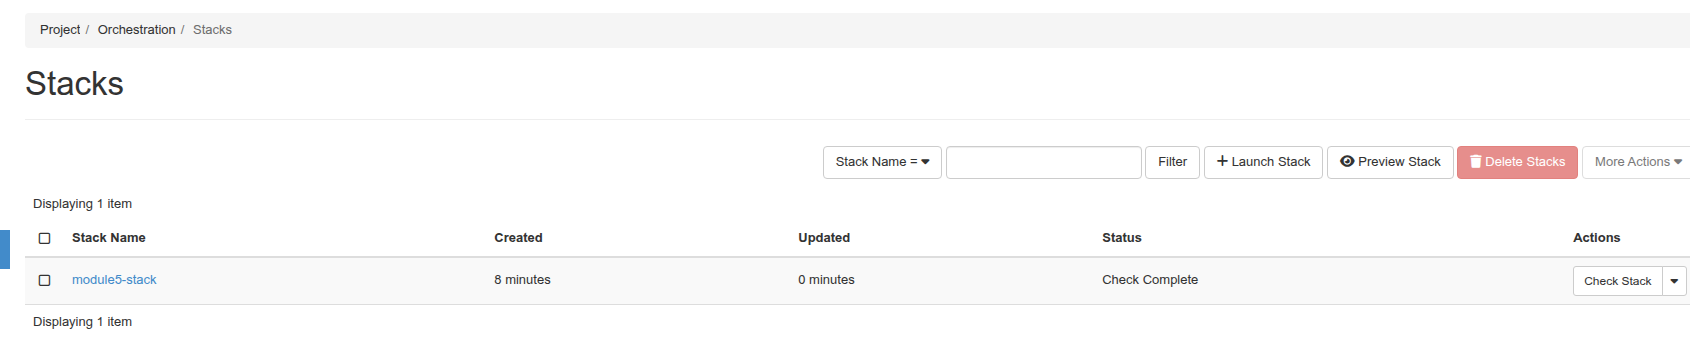
\includegraphics[width=0.88\linewidth]{img/m5-heat-stack-create-complete.png}
\caption{Heat stack \texttt{module5-stack} hoàn tất khởi tạo ở trạng thái thành công.}
\label{fig:m5_stack_status}
\end{figure}

\begin{figure}[H]
\centering
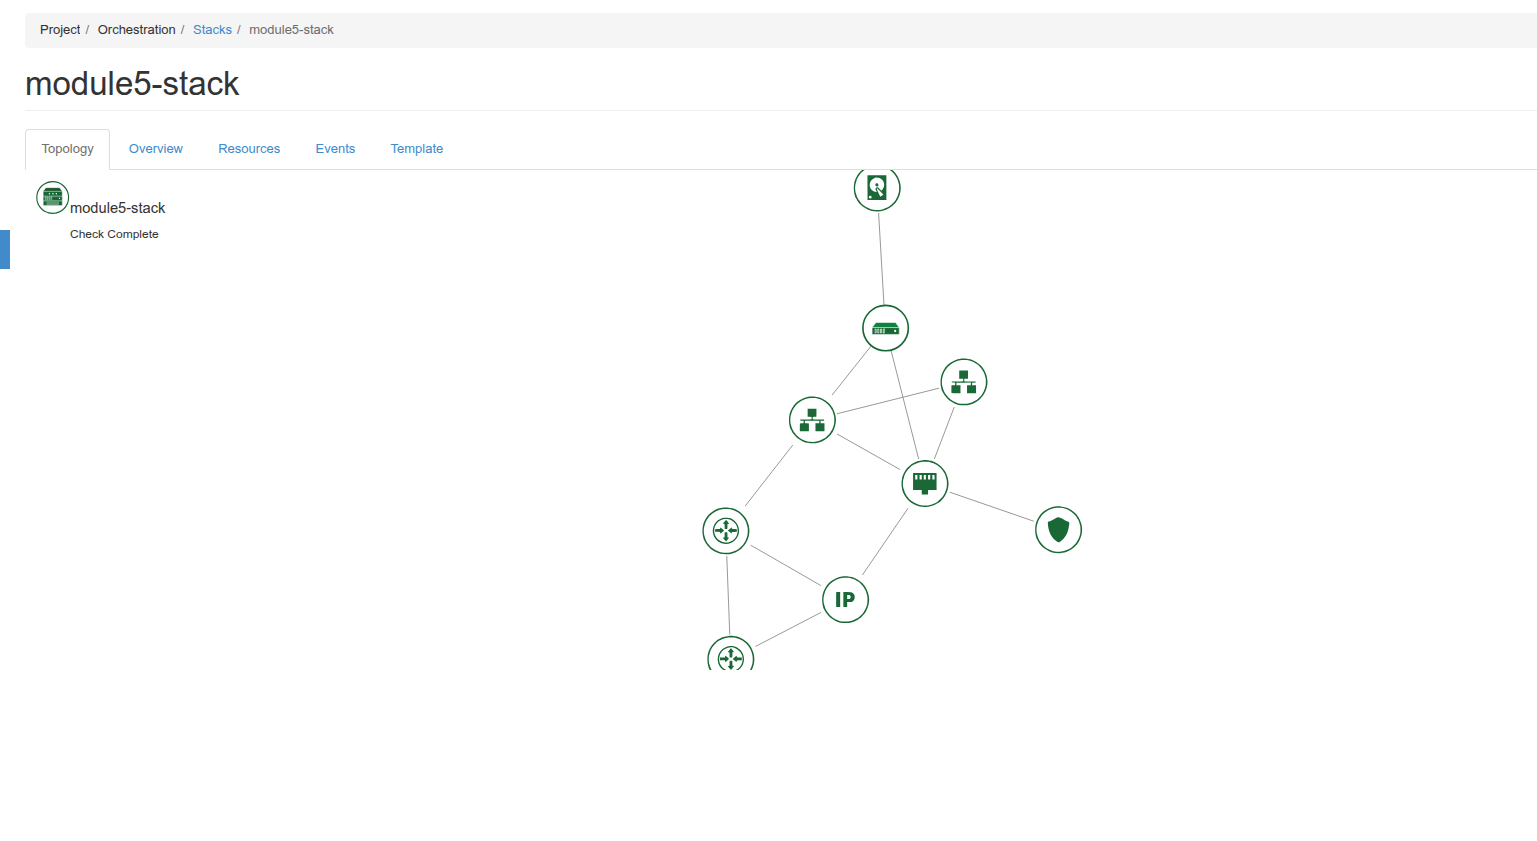
\includegraphics[width=0.88\linewidth]{img/m5-heat-stack-topology-graph.png}
\caption{Cây đồ thị phụ thuộc tài nguyên của Heat render trực quan trên Horizon.}
\label{fig:m5_stack_topology}
\end{figure}

Kết quả thực nghiệm cho thấy quy trình tự động hóa diễn ra chính xác và ổn định:
\begin{itemize}
    \item \textbf{Trạng thái Hoàn tất Cấp phát (Hình~\ref{fig:m5_stack_status}):} Heat Engine giải quyết thành công toàn bộ đồ thị phụ thuộc giữa các tài nguyên và chuyển stack sang trạng thái \texttt{CREATE\_COMPLETE} chỉ sau khoảng 60 giây.
    \item \textbf{Trực quan hóa Đồ thị Cấu trúc (Hình~\ref{fig:m5_stack_topology}):} Trên bảng điều khiển Horizon, cây topo tài nguyên hiển thị mạch lạc sự gắn kết giữa server, cổng mạng, nhóm bảo mật và volume lưu trữ theo đúng thiết kế khai báo.
    \item \textbf{Phân giải Tự động Đầu ra (Output Resolution):} Khối \texttt{outputs} của template tự động trả về đường dẫn URL công khai kèm địa chỉ Floating IP. Nhóm chúng em có thể truy cập ngay vào dịch vụ web qua trình duyệt mà không cần thêm bất kỳ thao tác cấu hình thủ công nào.
\end{itemize}


\newpage

\section{Nhật ký Sự cố Kỹ thuật \& Phân tích Nguyên nhân Gốc}

Quá trình xây dựng và vận hành hạ tầng đám mây OpenStack là một chuỗi thực nghiệm phức tạp, đòi hỏi sự phối hợp chính xác giữa nhiều tầng dịch vụ từ ảo hóa phần cứng, nhân Linux cho đến các giao thức mạng phân tán. Trong quá trình thực hiện đồ án, nhóm chúng em đã trực tiếp đối mặt và chẩn đoán nhiều sự cố kỹ thuật điển hình. Dưới đây là nhật ký chi tiết về 4 sự cố tiêu biểu, quy trình phân tích nguyên nhân gốc rễ (Root Cause Analysis - RCA) và phương án khắc phục triệt để mà nhóm chúng em đã đúc kết được:

\subsection{Sự cố 1: Lỗi HTTP 403 CSRF Forbidden trên Dashboard Horizon}
\begin{itemize}
    \item \textbf{Hiện tượng quan sát:} Khi nhóm chúng em truy cập giao diện quản trị Horizon từ xa thông qua đường hầm bảo mật HTTPS Reverse Proxy của NetBird (\url{https://openstack.net.selfhost.io.vn/dashboard}), trình duyệt lập tức bị từ chối truy cập với mã lỗi HTTP 403 Forbidden kèm thông báo: \textit{"CSRF verification failed. Request aborted."}
    \item \textbf{Phân tích nguyên nhân gốc:} Kể từ phiên bản Django 4.0 trở lên, cơ chế bảo vệ chống tấn công Cross-Site Request Forgery (CSRF) yêu cầu nghiêm ngặt tiêu đề HTTP \texttt{Origin} hoặc \texttt{Referer} của yêu cầu gửi đến phải khớp chính xác với danh sách định danh trong biến \texttt{CSRF\_TRUSTED\_ORIGINS}. Cấu hình mặc định của DevStack chỉ cho phép truy cập cục bộ qua \texttt{localhost} và địa chỉ IP trực tiếp của máy chủ vật lý (\texttt{192.168.2.10}), dẫn đến việc mọi yêu cầu đi qua tên miền proxy bên ngoài đều bị chặn lại.
    \item \textbf{Giải pháp khắc phục:} Nhóm chúng em đã tiến hành bổ sung tên miền NetBird kèm cả hai giao thức (\texttt{https://} và \texttt{http://}) vào tệp cấu hình \nolinkurl{/etc/openstack-dashboard/local_settings.py}, sau đó khởi động lại dịch vụ web server Apache:
\begin{lstlisting}[language=python]
CSRF_TRUSTED_ORIGINS = [
    'https://openstack.net.selfhost.io.vn',
    'http://openstack.net.selfhost.io.vn',
    'http://192.168.2.10'
]
\end{lstlisting}
\end{itemize}

\subsection{Sự cố 2: Rớt gói tin do Định tuyến Bất đối xứng trên Máy ảo Dual-NIC}
\begin{itemize}
    \item \textbf{Hiện tượng quan sát:} Sau khi gán địa chỉ Floating IP \texttt{172.24.4.187} vào cổng DMZ của máy ảo 2 card mạng (\texttt{module3-web-sever}), nhóm chúng em nhận thấy máy khách ngoài Internet có thể gửi lệnh ICMP Ping thành công nhưng mọi kết nối HTTP GET trên cổng 80 đều bị treo (timeout) và không thể tải được trang web.
    \item \textbf{Phân tích nguyên nhân gốc:} Do máy ảo được cấp phát 2 card mạng (\texttt{eth0} thuộc mạng Private và \texttt{eth1} thuộc mạng DMZ), tiến trình DHCP client trong hệ điều hành máy ảo tự động tạo ra 2 tuyến đường mặc định (Default Gateway) có cùng mức ưu tiên (metric). Khi máy khách gửi gói tin TCP SYN vào cổng DMZ (\texttt{eth1}), máy chủ phản hồi gói TCP SYN-ACK nhưng kernel lại đẩy gói tin ra qua cổng \texttt{eth0} theo bảng định tuyến mặc định. Vì gói tin chiều ra đi vòng qua cổng Private thay vì cổng DMZ (nơi Router L3 đang duy trì bảng theo dõi trạng thái phiên kết nối Netfilter Conntrack/DNAT), Router L3 đã chủ động hủy bỏ gói tin do vi phạm tính đối xứng trạng thái (Asymmetric Routing Drop).
    \item \textbf{Giải pháp khắc phục:} Nhóm chúng em đã can thiệp trực tiếp vào bảng định tuyến nhân Linux của máy ảo, xóa tuyến đường mặc định trên \texttt{eth0} và thiết lập tuyến đường qua cổng DMZ (\texttt{eth1}) có mức ưu tiên cao nhất:
\begin{lstlisting}[language=bash]
$ sudo ip route replace default via 10.10.10.1 dev eth1 metric 100
$ sudo ip route del default via 10.10.20.1 dev eth0
\end{lstlisting}
\end{itemize}

\subsection{Sự cố 3: Máy ảo không thể kết nối tới Swift API từ Subnet Private}
\begin{itemize}
    \item \textbf{Hiện tượng quan sát:} Khi thực hiện kịch bản tải mã nguồn từ Swift về máy ảo nằm trong phân đoạn mạng nội bộ, tiến trình \texttt{wget} liên tục báo lỗi \textit{"Connection refused"} hoặc timeout khi cố gắng kết nối tới cổng 8080.
    \item \textbf{Phân tích nguyên nhân gốc:} Dịch vụ Swift Proxy được DevStack cấu hình lắng nghe trên địa chỉ IP của card mạng quản trị máy chủ vật lý (\texttt{192.168.2.10:8080}). Do máy ảo nằm trong subnet cô lập không có đường nối trực tiếp tới dải mạng quản trị của host, các gói tin yêu cầu bị mắc kẹt tại router ảo do thiếu cờ chuyển tiếp gói tin (IP Forwarding) trên hệ điều hành host và thiếu tuyến Gateway ngoại vi thích hợp trên L3 Router.
    \item \textbf{Giải pháp khắc phục:} Nhóm chúng em đã kích hoạt cờ \texttt{net.ipv4.ip\_forward=1} trên máy chủ vật lý, đồng thời cấu hình định tuyến thông qua Gateway ngoại vi của Neutron Router để cho phép máy ảo gửi gói tin trực tiếp tới endpoint Swift của host.
\end{itemize}

\subsection{Sự cố 4: Race Condition khi Đính kèm Ổ đĩa VirtIO trong Cloud-Init}
\begin{itemize}
    \item \textbf{Hiện tượng quan sát:} Trong các lần thực thi tự động hóa với OpenStack Heat, nhóm chúng em ghi nhận xác suất ngẫu nhiên stack gặp lỗi khởi tạo hoặc dịch vụ web không hoạt động. Kiểm tra nhật ký \texttt{/var/log/cloud-init-output.log} cho thấy lệnh \texttt{mkfs.ext4 /dev/vdb} bị gián đoạn với thông báo: \textit{"Device does not exist"}.
    \item \textbf{Phân tích nguyên nhân gốc:} Đây là hiện tượng tương tranh thời gian (Race Condition) kinh điển giữa tiến trình ảo hóa tính toán và lưu trữ: máy ảo Nova khởi động cực nhanh và Cloud-Init thực thi script \texttt{user\_data} gần như tức thì, trong khi tiến trình Cinder/QEMU gửi lệnh hot-plug ổ đĩa ảo qua socket điều khiển có độ trễ nhất định. Tại thời điểm script gọi lệnh format, kernel Linux chưa kịp nạp driver \texttt{virtio\_blk} cho thiết bị \texttt{/dev/vdb}.
    \item \textbf{Giải pháp khắc phục:} Nhóm chúng em đã tái cấu trúc đoạn mã khởi tạo trong Cloud-Init, bổ sung một vòng lặp chủ động thăm dò (polling loop) kiểm tra sự hiện diện của thiết bị khối kèm cơ chế kiểm tra idempotent với \texttt{blkid} trước khi tiến hành định dạng:
\begin{lstlisting}[language=bash]
for i in {1..30}; do
    [ -b /dev/vdb ] && break
    sleep 2
done
blkid /dev/vdb || mkfs.ext4 /dev/vdb
\end{lstlisting}
\end{itemize}

\newpage

\section{Tổng kết \& Đánh giá Đồ án}

\subsection{So sánh Vận hành Thủ công vs Tự động hóa Heat}
Thông qua quá trình triển khai thực tế toàn bộ 5 module, nhóm chúng em đã tiến hành đo đạc và đối chiếu thực nghiệm giữa hai phương pháp quản trị hạ tầng trên OpenStack: phương pháp thực thi thủ công theo từng bước mệnh lệnh (Imperative Approach) và phương pháp tự động hóa khai báo với Heat Orchestration (Declarative IaC Approach). Bảng~\ref{tab:comparison} tổng hợp chi tiết các chỉ số và đặc tính vận hành giữa hai mô hình:

\begin{table}[H]
\centering
\small
\begin{tabularx}{\linewidth}{|l|>{\raggedright\arraybackslash}X|>{\raggedright\arraybackslash}X|}
\hline
\textbf{Tiêu chí Đánh giá} & \textbf{Vận hành Thủ công (Mod 1--4)} & \textbf{Điều phối Heat (Mod 5)} \\ \hline
Thời gian Cấp phát & 15--25 phút (nhiều bước qua CLI/Horizon) & $\approx 60$ giây (1 lệnh \texttt{openstack stack create}) \\ \hline
Tỷ lệ Sai sót Con người & Cao (dễ nhầm IP, sai gateway, thiếu rule SG) & Gần như triệt tiêu (khai báo chuẩn hóa, có tính Idempotent) \\ \hline
Thu hồi Tài nguyên & Phức tạp, bắt buộc xóa ngược thứ tự phụ thuộc & Tối giản, tự động giải phóng qua 1 lệnh (\texttt{stack delete}) \\ \hline
Quản lý Phiên bản & Lịch sử dòng lệnh rời rạc, khó lưu vết & Template YAML có cấu trúc, quản lý tập trung qua Git \\ \hline
Khả năng Tái lập & Khó nhân bản chính xác trên môi trường mới & Tái lập môi trường tức thì chỉ với một tệp tham số \\ \hline
\end{tabularx}
\caption{So sánh đặc tính vận hành giữa phương pháp thủ công và tự động hóa khai báo với Heat.}
\label{tab:comparison}
\end{table}

\subsection{Tổng kết Kết quả Đạt được}
Đồ án đã giúp nhóm chúng em hoàn thành toàn diện và xuất sắc tất cả các mục tiêu kỹ thuật đề ra ban đầu:
\begin{enumerate}
    \item \textbf{Làm chủ Hạ tầng Đám mây Cốt lõi:} Xây dựng thành công hệ thống đám mây riêng OpenStack tích hợp đầy đủ năng lực tính toán (Nova), mạng điều khiển bằng phần mềm (Neutron), lưu trữ khối (Cinder), lưu trữ đối tượng (Swift) và điều phối tự động (Heat).
    \item \textbf{Thiết kế Mạng Đa tầng Bảo mật:} Hiện thực hóa kiến trúc mạng doanh nghiệp phân vùng nghiêm ngặt giữa dải mạng DMZ công khai và dải mạng Private nội bộ, kiểm soát luồng dữ liệu an toàn qua Router L3 và Floating IP.
    \item \textbf{Giải quyết Triệt để Bài toán Định tuyến Phức tạp:} Chẩn đoán và xử lý thành công hiện tượng rớt gói tin do định tuyến bất đối xứng (Asymmetric Routing) trên máy ảo đa card mạng, làm chủ cơ chế theo dõi trạng thái phiên kết nối Netfilter Conntrack của nhân Linux.
    \item \textbf{Hiện thực hóa Mô hình Lưu trữ Doanh nghiệp:} Triển khai hiệu quả mô hình lưu trữ lai kết hợp giữa Swift và Cinder, đồng thời kiểm chứng thành công quy trình sao lưu và phục hồi thảm họa tức thời thông qua Volume Snapshot với độ toàn vẹn dữ liệu đạt 100\%.
    \item \textbf{Tự động hóa Toàn diện với IaC:} Chuẩn hóa toàn bộ hạ tầng thành mã nguồn mẫu Heat Orchestration Template (HOT), kết hợp cùng kịch bản Cloud-Init có tính Idempotent để tự động hóa trọn gói quá trình cấp phát và triển khai dịch vụ mà không cần bất kỳ can thiệp thủ công nào.
\end{enumerate}

\subsection{Bài học Kinh nghiệm \& Hướng Phát triển}
\noindent \textbf{Bài học Kinh nghiệm Thực tiễn:}
Qua quá trình trực tiếp triển khai và xử lý sự cố trên OpenStack, nhóm chúng em đã đúc kết được những kinh nghiệm thực tế quý giá:
\begin{itemize}
    \item Tầm quan trọng của việc hiểu sâu cơ chế mạng ở tầng nhân Linux (Kernel Routing, IPTables, Conntrack) khi vận hành các hệ thống ảo hóa đa cổng mạng.
    \item Nhận thức rõ sự khác biệt giữa các mô hình lưu trữ (Block vs Object) để lựa chọn giải pháp tối ưu cho từng loại dữ liệu ứng dụng.
    \item Kỹ năng phòng ngừa và xử lý các vấn đề tương tranh thời gian (Race Condition) trong môi trường tự động hóa phân tán.
\end{itemize}

\noindent \textbf{Hướng Phát triển Mở rộng:}
Dựa trên nền tảng hạ tầng đã xây dựng thành công, đồ án có thể tiếp tục được mở rộng theo các hướng nghiên cứu ứng dụng chuyên sâu:
\begin{itemize}
    \item \textbf{Tích hợp Đường ống CI/CD:} Kết nối Heat template với GitLab CI / GitHub Actions để tự động hóa quy trình kiểm thử và triển khai hạ tầng liên tục (GitOps).
    \item \textbf{Mở rộng Công cụ IaC Đa nền tảng:} Thử nghiệm chuyển dịch từ Heat sang Terraform và Ansible nhằm nâng cao tính linh hoạt và khả năng quản lý hạ tầng đa đám mây (Multi-Cloud).
    \item \textbf{Nền tảng Điều phối Container (Kubernetes on OpenStack):} Khởi tạo cụm Kubernetes trên các máy ảo OpenStack thông qua OpenStack Magnum, xây dựng hạ tầng sẵn sàng cho các ứng dụng kiến trúc Microservices hiện đại.
\end{itemize}

\newpage

\bibliographystyle{IEEEtran}
\bibliography{references}

\end{document}

